% Chapter 2 — System Components and Design
% Input this file from the main document, which must have in its preamble:
%   \usepackage{listings}  \usepackage{xcolor}  \usepackage{amsmath}
%   \usepackage{amssymb}   \usepackage{booktabs} \usepackage{array}
%   \usepackage{placeins}  \usepackage{enumitem} \usepackage{caption}
%   \usepackage{needspace} \usepackage{etoolbox} \usepackage{setspace}
%   \usepackage{tikz}
%   \usetikzlibrary{positioning, arrows.meta, fit, backgrounds}
%
% Also define in preamble (or here once):
%   \definecolor{codebg}{HTML}{F5F5F5}
%   \definecolor{codeframe}{HTML}{CCCCCC}
%   \definecolor{codecomment}{HTML}{6A737D}
%   \definecolor{codestring}{HTML}{032F62}
%   \definecolor{codekeyword}{HTML}{D73A49}
%   \lstdefinestyle{clean}{...}  (see below)
%   \newcommand{\code}[1]{\texttt{#1}}

\definecolor{codebg}{HTML}{F5F5F5}
\definecolor{codeframe}{HTML}{CCCCCC}
\definecolor{codecomment}{HTML}{6A737D}
\definecolor{codestring}{HTML}{032F62}
\definecolor{codekeyword}{HTML}{D73A49}

\lstdefinestyle{clean}{
    backgroundcolor=\color{codebg},
    basicstyle=\ttfamily\small\linespread{1.1}\selectfont,
    breaklines=true,
    breakatwhitespace=true,
    frame=single,
    framerule=0.4pt,
    rulecolor=\color{codeframe},
    xleftmargin=0.75em,
    xrightmargin=0.75em,
    aboveskip=0.8em,
    belowskip=0.8em,
    showstringspaces=false,
    tabsize=4,
    commentstyle=\color{codecomment}\itshape,
    keywordstyle=\color{codekeyword}\bfseries,
    stringstyle=\color{codestring},
    extendedchars=true,
    keepspaces=true,
    captionpos=b,
    numbers=none,
}
\lstset{style=clean}

\providecommand{\code}[1]{\texttt{#1}}
\usetikzlibrary{positioning, arrows.meta, fit, backgrounds}

\makeatletter
\titleformat{\chapter}[block]
  {\normalfont\huge\bfseries\color{ImperialBlue}}
  {\thechapter}{20pt}{\huge}
\titlespacing*{\chapter}{0pt}{-20pt}{15pt}
\makeatother

\titlespacing*{\paragraph}{0pt}{0.4ex}{0.2ex}

\chapter{System Components and Design}
\label{ch2}

\begin{spacing}{0.3}
\minitoc
\end{spacing}

\thesisspacing


% ===============================================================
\section{System Overview}
% ===============================================================

This chapter gives a detailed breakdown of each hardware and software subsystem,
with a mathematically rigorous treatment of ray marching and the custom
arithmetic that makes it feasible in hardware. Figure~\ref{fig:system_arch}
shows the full system architecture.

The rendering pipeline is a deeply pipelined hardware datapath on the
programmable logic (PL). Pixel coordinates enter \code{pixel\_dispatch}, flow
through ray generation (48 cycles), enter the SDF evaluation stage inside
\code{march\_core} (107 cycles), advance along the ray in the step unit (8
cycles), and either terminate (hit or max iterations) or re-enter the pipeline
via \code{feedback\_ctrl} for another sphere-tracing iteration. Completed pixels
are burst to DDR3 by the AXI framebuffer writer, and the VDMA IP streams the
completed frame to the HDMI display at $1024\times600$ pixels.

Two independent input streams modulate the scene in real time. \textbf{Camera
orientation} is supplied by an MPU-6050 inertial measurement unit connected to
the PS over I$^2$C. Raw accelerometer and gyroscope readings are fused in a
complementary filter running on the ARM Cortex-A9 (\code{ctrl.py}) to produce
pitch, roll, and yaw estimates. These are used to construct a $3\times3$ lookat
matrix, which is written each frame to the AXI-Lite camera register file at
\texttt{0x43C00000} alongside the camera origin. \textbf{Music reactivity} is
supplied by a 1024-point FFT pipeline running on the host PC. Per audio block,
bass, mid, and treble energy bands, RMS, spectral centroid, zero-crossing rate,
and a beat detection flag are computed and streamed over TCP. The PS receives
these eleven features and writes them directly into the AXI-Lite SDF parameter
registers, where the PL picks them up at the start of each SDF evaluation.

\begin{figure}[htbp]
\centering
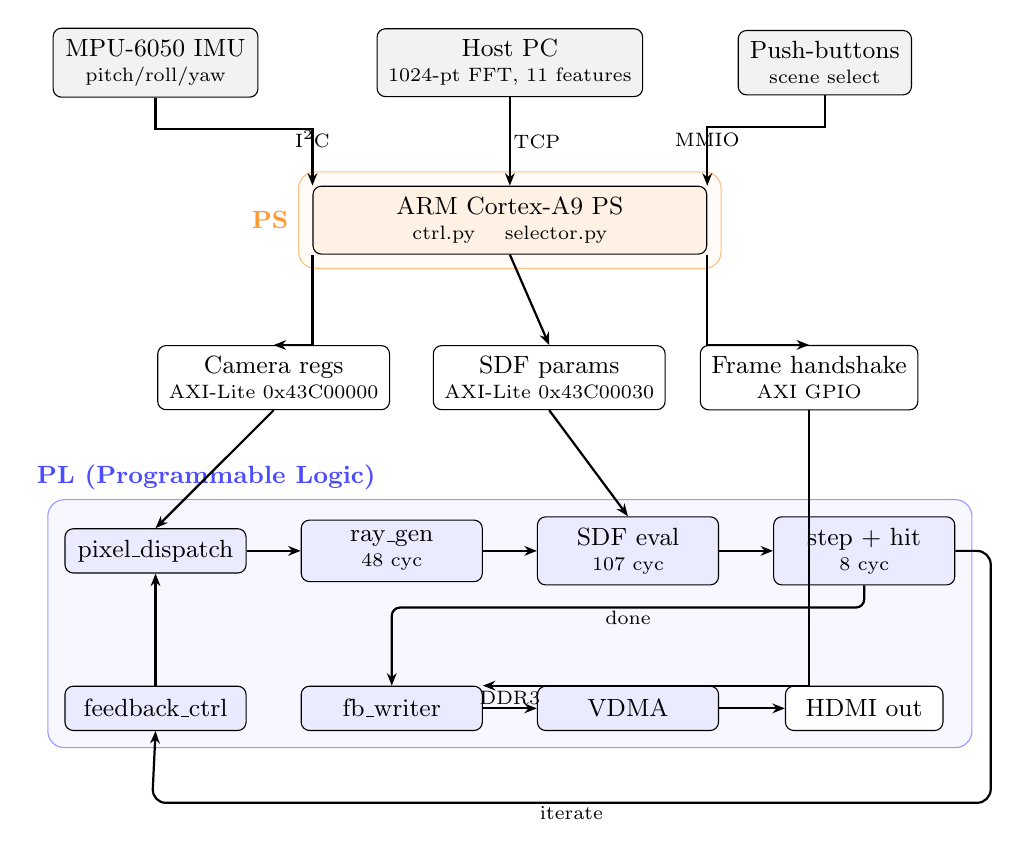
\begin{tikzpicture}[
    box/.style   ={draw, rounded corners=3pt, align=center,
                   minimum height=1.6em, inner sep=4pt, font=\small, fill=white},
    extbox/.style={box, fill=gray!10},
    psbox/.style ={box, fill=orange!10},
    plbox/.style ={box, fill=blue!8},
    arr/.style   ={-{Stealth[length=4.5pt, width=3.5pt]}, thick},
    lbl/.style   ={font=\scriptsize, inner sep=1pt}
]

%% ── External sources (top row) ───────────────────────────────────
\node[extbox, minimum width=2.6cm] (imu)    at (0,    0)
    {MPU-6050 IMU\\[-2pt]{\scriptsize pitch/roll/yaw}};
\node[extbox, minimum width=2.6cm] (hostpc) at (4.5,  0)
    {Host PC\\[-2pt]{\scriptsize 1024-pt FFT, 11 features}};
\node[extbox, minimum width=2.2cm] (btns)   at (8.5,  0)
    {Push-buttons\\[-2pt]{\scriptsize scene select}};

%% ── PS ───────────────────────────────────────────────────────────
\node[psbox, minimum width=5.0cm] (ps) at (4.5, -2.0)
    {ARM Cortex-A9 PS\\[-2pt]{\scriptsize ctrl.py \quad selector.py}};

%% ── AXI register interfaces ──────────────────────────────────────
\node[box, minimum width=2.8cm] (camregs) at (1.5, -4.0)
    {Camera regs\\[-2pt]{\scriptsize AXI-Lite 0x43C00000}};
\node[box, minimum width=2.8cm] (sdfp)    at (5.0, -4.0)
    {SDF params\\[-2pt]{\scriptsize AXI-Lite 0x43C00030}};
\node[box, minimum width=2.6cm] (gpiohsk) at (8.3, -4.0)
    {Frame handshake\\[-2pt]{\scriptsize AXI GPIO}};

%% ── PL pipeline row 1 ────────────────────────────────────────────
\node[plbox, minimum width=2.3cm] (dispatch) at (0,   -6.2)
    {pixel\_dispatch};
\node[plbox, minimum width=2.3cm] (rg)       at (3.0, -6.2)
    {ray\_gen\\[-2pt]{\scriptsize 48 cyc}};
\node[plbox, minimum width=2.3cm] (sdfev)    at (6.0, -6.2)
    {SDF eval\\[-2pt]{\scriptsize 107 cyc}};
\node[plbox, minimum width=2.3cm] (steph)    at (9.0, -6.2)
    {step + hit\\[-2pt]{\scriptsize 8 cyc}};

%% ── PL pipeline row 2 (feedback + output) ────────────────────────
\node[plbox, minimum width=2.3cm] (fbctrl)  at (0,   -8.2)
    {feedback\_ctrl};
\node[plbox, minimum width=2.3cm] (fbwrite) at (3.0, -8.2)
    {fb\_writer};
\node[plbox, minimum width=2.3cm] (vdma)    at (6.0, -8.2)
    {VDMA};
\node[box,   minimum width=2.0cm] (hdmi)    at (9.0, -8.2)
    {HDMI out};

%% ── External → PS ────────────────────────────────────────────────
\draw[arr] (imu.south)  -- ++(0,-0.4) -| node[lbl, above, pos=0.7]{I$^2$C} (ps.north west);
\draw[arr] (hostpc)     -- node[lbl, right]{TCP} (ps.north);
\draw[arr] (btns.south) -- ++(0,-0.4) -| node[lbl, above, pos=0.7]{MMIO}   (ps.north east);

%% ── PS → AXI interfaces ──────────────────────────────────────────
\draw[arr] (ps.south west) |- (camregs.north);
\draw[arr] (ps.south)      -- (sdfp.north);
\draw[arr] (ps.south east) |- (gpiohsk.north);

%% ── AXI → PL ─────────────────────────────────────────────────────
\draw[arr] (camregs.south) -- (dispatch.north);
\draw[arr] (sdfp.south)    -- (sdfev.north);
\draw[arr] (gpiohsk.south) |- (fbwrite.north east);

%% ── Pipeline datapath ────────────────────────────────────────────
\draw[arr] (dispatch) -- (rg);
\draw[arr] (rg)       -- (sdfev);
\draw[arr] (sdfev)    -- (steph);

%% ── Done pixels: steph → fbwrite (route through gap between rows)
\draw[arr, rounded corners=3pt]
    (steph.south) -- ++(0,-0.28)
    -- node[lbl, below]{done} ++(-6.0,0)
    -- (fbwrite.north);

%% ── Iterate: steph → loop around right → fbctrl.south ──────────
\draw[arr, rounded corners=5pt]
    (steph.east) -- ++(0.45,0) -- ++(0,-3.2)
    -- node[lbl, below]{iterate} ++(-10.65,0)
    -- (fbctrl.south);

%% ── fbctrl feeds back to dispatch ───────────────────────────────
\draw[arr] (fbctrl.north) -- (dispatch.south);

%% ── Output path ──────────────────────────────────────────────────
\draw[arr] (fbwrite) -- node[lbl, above]{DDR3} (vdma);
\draw[arr] (vdma)    -- (hdmi);

%% ── Background shading ───────────────────────────────────────────
\begin{scope}[on background layer]
    \node[draw=blue!40, fill=blue!3, rounded corners=6pt,
          inner sep=6pt,
          fit=(dispatch)(rg)(sdfev)(steph)(fbctrl)(fbwrite)(vdma)(hdmi),
          label={[font=\small\bfseries, text=blue!70]above left:PL (Programmable Logic)}
    ] {};
    \node[draw=orange!50, fill=orange!3, rounded corners=6pt,
          inner sep=5pt,
          fit=(ps),
          label={[font=\small\bfseries, text=orange!80]left:PS}
    ] {};
\end{scope}

\end{tikzpicture}
\caption{Full system architecture, more on this in Section 3, Integration. IMU and host-PC FFT
feed the ARM PS, which programs the PL over AXI-Lite each frame. The PL pipeline traces rays in a
feedback loop and streams completed frames to HDMI via VDMA.}
\label{fig:system_arch}
\end{figure}

\FloatBarrier


% ===============================================================
\section{Custom 27-bit Floating-Point Format}
\label{sec:fp}
% ===============================================================

\subsection{Format and Motivation}

The entire hardware rendering pipeline uses a custom 27-bit floating-point
format rather than IEEE\,754 single precision (32-bit) or fixed-point arithmetic.
The format is \texttt{\{sign[26], exponent[25:18], mantissa[17:0]\}}: one sign
bit, an eight-bit biased exponent identical to IEEE\,754 (bias 127), and an
eighteen-bit mantissa with an implicit leading 1. This gives the same dynamic
range as IEEE\,754 single precision with exponents from $2^{-126}$ to $2^{127}$ 
while reducing the word width by five bits.

\begin{table}[htbp]
\centering
\small
\caption{Floating-point formats across the project}
\label{tab:fp_formats}
{\renewcommand{\arraystretch}{1.4}
\begin{tabular}{lcccc}
\toprule
\textbf{Format} & \textbf{Sign} & \textbf{Exponent} & \textbf{Mantissa} & \textbf{Total} \\
\midrule
IEEE-754 float32       & 1 & 8     & 23      & 32 bits \\
Project FP27           & 1 & 8     & 18      & 27 bits \\
Q4.12 (neural weights) & 1 & 4 int & 12 frac & 16 bits \\
\bottomrule
\end{tabular}}
\end{table}

\FloatBarrier

\subsection{Bit Layout and Worked Conversions}

Figure~\ref{fig:fp27_bits} shows the 27-bit field breakdown. The exponent is
biased at 127 (= \texttt{0b01111111}) so that the zero exponent is represented
as \texttt{0b10000000}, matching IEEE\,754 and allowing the same exponent
arithmetic ie negative exponents as well as positive exponents. The mantissa carries an implicit leading 1 bit, so the full
represented mantissa is $1.m_{17}m_{16}\cdots m_0$.

\begin{figure}[htbp]
\centering
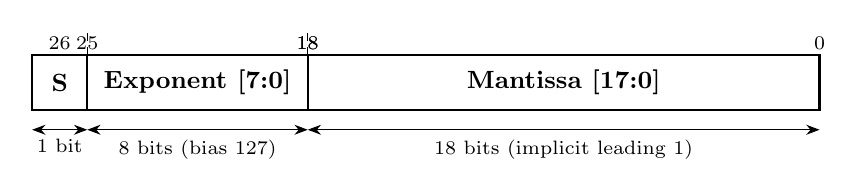
\begin{tikzpicture}[font=\small]
    % Bit-field rectangles
    \draw[thick] (0,0) rectangle (0.7, 0.7);   % bit 26: sign
    \draw[thick] (0.7,0) rectangle (3.5, 0.7); % bits 25:18 exponent (8 bits)
    \draw[thick] (3.5,0) rectangle (10.0, 0.7);% bits 17:0 mantissa (18 bits)

    % Labels inside boxes
    \node at (0.35, 0.35) {\textbf{S}};
    \node at (2.1,  0.35) {\textbf{Exponent [7:0]}};
    \node at (6.75, 0.35) {\textbf{Mantissa [17:0]}};

    % Bit indices above
    \node[font=\scriptsize] at (0.35, 0.85) {26};
    \node[font=\scriptsize] at (0.7,  0.85) {25};
    \node[font=\scriptsize] at (3.5,  0.85) {18};
    \node[font=\scriptsize] at (3.5,  0.85) {18};
    \node[font=\scriptsize] at (10.0, 0.85) {0};
    \draw[densely dashed] (0.7, 0.7) -- (0.7, 1.0);
    \draw[densely dashed] (3.5, 0.7) -- (3.5, 1.0);

    % Width annotations below
    \draw[<->, >=Stealth] (0, -0.25) -- node[below, font=\scriptsize]{1 bit} (0.7, -0.25);
    \draw[<->, >=Stealth] (0.7, -0.25) -- node[below, font=\scriptsize]{8 bits (bias 127)} (3.5, -0.25);
    \draw[<->, >=Stealth] (3.5, -0.25) -- node[below, font=\scriptsize]{18 bits (implicit leading 1)} (10.0, -0.25);
\end{tikzpicture}
\caption{FP27 bit field layout: 1 sign, 8 exponent (bias 127), 18 mantissa.}
\label{fig:fp27_bits}
\end{figure}

\FloatBarrier

\paragraph{Converting a decimal value to FP27.}\newline
As a concrete example, convert $-3.5$ to FP27.
\begin{enumerate}[noitemsep]
    \item \textbf{Sign:} negative $\implies s = 1$.
    \item \textbf{Exponent:} $3.5 = 1.75 \times 2^1$, so the unbiased exponent
          is $1$, and the stored exponent is $e = 127 + 1 = 128 =
          \texttt{0b10000000}$.
    \item \textbf{Mantissa:} the fractional part is $0.75$. In binary:
          $0.75 = 0.11_2$, giving mantissa bits $m = \texttt{11\,0000\,0000\,0000\,0000}$
          ($0.75 \times 2^{18} = 196608 = \texttt{0x30000}$).
    \item \textbf{Result:}
          \[
              \texttt{1\_10000000\_110000000000000000} = \texttt{27'hC30000}
          \]
\end{enumerate}

\paragraph{Converting FP27 back to decimal.}\newline
Given \texttt{27'h1E40000}: $s{=}0$, $e{=}\texttt{0x3C}{=}60$, $m{=}\texttt{0x40000}{=}262144$.
\[
    \text{value} = (-1)^0 \times (1 + 262144/2^{18}) \times 2^{60-127}
    = 1.5 \times 2^{-67} \approx 1.02 \times 10^{-20}
\]
This illustrates the extreme dynamic range the format provides: representing
$\sim 10^{-20}$ exactly is impossible in Q2.29 fixed point but trivial in FP27.

\paragraph{Conversion from IEEE\,754 in software.}\newline
The Python controller uses the following to pack FP27 values into AXI registers
(truncating the bottom 5 mantissa bits):
\begin{lstlisting}[language=Python]
def fp32_to_fp27(value):
    bits      = struct.unpack(">I", struct.pack(">f", float(value)))[0]
    sign      = (bits >> 31) & 0x1
    exponent  = (bits >> 23) & 0xFF      # same 8-bit biased exponent
    frac23    = bits & 0x7FFFFF
    frac18    = (frac23 + 0x10) >> 5     # round, then drop bottom 5 bits
    return (sign << 26) | (exponent << 18) | frac18
\end{lstlisting}
The exponent is identical between IEEE\,754 and FP27 (same bias, same width), so
no conversion is needed there --- only the mantissa is truncated.

\paragraph{Why not fixed-point? }\mbox{}\newline
Ray marching requires evaluating distances that span several orders of magnitude
in a single frame. The hit threshold is approximately $10^{-3}$ (a ray is
considered to have struck a surface when the SDF returns a value smaller than
this); the maximum step size can reach several scene units. A fixed-point format
must accommodate both extremes simultaneously. The Q2.29 format used in early
RTL could only represent values in $[-2, 2]$, which immediately constrained
scene scale and caused precision collapse as distances accumulated over 128
iterations. Floating-point represents each value relative to its own magnitude,
so small distances near surfaces remain precise regardless of how far the ray
has travelled.

\paragraph{Why 27 bits, not 32?}\mbox{}\newline
The Xilinx PYNQ-Z1 contains DSP48E1 slices whose multiplier operates on
$18 \times 25$ bit inputs. IEEE\,754 single precision requires a $24 \times 24$
bit mantissa multiply (including the implicit leading bit), which exceeds the
18-bit input port and forces Vivado to cascade two DSP blocks per multiply. With
an 18-bit mantissa, the product $(1.\text{mantissa}) \times (1.\text{mantissa})$
fits in one DSP48E1 exactly: the 19-bit inputs ($1 +$ 18 mantissa bits) produce
a 38-bit product, which is truncated to 18 bits after normalisation. Using
27-bit FP therefore halves the DSP count per multiply relative to IEEE\,754,
directly determining whether the design fits on chip. The five mantissa bits
sacrificed cause a maximum relative error of $2^{-18} \approx 3.8 \times
10^{-6}$, which is invisible at $1024 \times 600$ or $512 \times 300$ pixel
resolution. The mantissa carries an implicit leading 1, which comes at the cost
of not being able to represent subnormal numbers. Given our purpose (real-time
psychedelic renders, not pixel-perfect scientific computation) this was an
explicit decision not to pursue subnormals. This follows traditional baseline
GPU architecture: subnormal handling typically requires a kernel trap to the CPU
which is an extensive overhead and is omitted in most GPU shader cores for the same
reason.


% ===============================================================
\section{Floating-Point Library}
\label{sec:fplibrary}
% ===============================================================

\subsection{Library Overview}

The FP library comprises 16 fully pipelined synthesisable Verilog modules,
each accepting a new input every clock cycle and producing a result after a
fixed latency with no stall or handshake signals. Pipeline synchronisation
between modules of differing latencies is handled exclusively by
\code{state\_pipe} delay lines. SRT division and Goldschmidt's algorithm were
evaluated before settling on Newton-Raphson reciprocal for its fixed-latency
amenability.

\begin{table}[htbp]
\centering
\small
\caption{27-bit FP library modules and pipeline latencies}
\label{tab:fp_lib}
{\renewcommand{\arraystretch}{1.3}
\begin{tabular}{llc}
\toprule
\textbf{Module} & \textbf{Operation} & \textbf{Latency (cycles)} \\
\midrule
\code{fp\_mul.v}            & Multiply                            & 4  \\
\code{fp\_add.v}            & Add                                 & 4  \\
\code{fp\_sub.v}            & Subtract                            & 4  \\
\code{fp\_inverse.sv}       & $1/b$ via Newton-Raphson            & 36 \\
\code{fp\_division.sv}      & $a/b = a \times (1/b)$              & 40 \\
\code{fp\_isqrt.v}          & $1/\sqrt{x}$ via NR + magic number  & 16 \\
\code{fp\_length.v}         & $\|\mathbf{v}\|$                    & 32 \\
\code{fp\_modulus.sv}       & $a \bmod b$ for space repetition    & 52 \\
\code{fp\_floor.sv}         & $\lfloor a \rfloor$ (combinational) & 0  \\
\code{fp\_abs.v}            & $|a|$ (combinational)               & 0  \\
\code{fp\_negate.v}         & $-a$ (combinational)                & 0  \\
\code{fp\_min.v}            & $\min(a,b)$ (combinational)         & 0  \\
\code{fp\_max.v}            & $\max(a,b)$ (combinational)         & 0  \\
\code{int2fp.v}             & Integer $\to$ FP27                  & 1  \\
\code{fp\_normalize.sv}     & Normalise FP27 vector               & 8  \\
\code{fp\_mul\_vec3\_mat33.sv} & $3\times3$ matrix $\times$ vector & 8  \\
\bottomrule
\end{tabular}}
\end{table}

\FloatBarrier

\subsection{Multiplication - \code{fp\_mul.v}}

Two FP27 numbers $a$ and $b$ are multiplied as:
\[
    \text{sign} = a_s \oplus b_s, \quad
    \text{exp} = e_a + e_b - 127, \quad
    \text{mant} = (1.m_a) \times (1.m_b)
\]
The $19\times19$-bit mantissa product yields 38 bits; overflow (product $\geq
2$) shifts the mantissa right and increments the exponent. The four-stage
pipeline is: (1) register inputs; (2) DSP48E1 multiply with
\lstinline[language=Verilog]{(* use_dsp = "yes" *)}; (3) register raw DSP
output, breaking the carry chain from normalisation; (4) normalise and
propagate zero flag. Stage 3 is critical: without it, the normalisation mux
sits combinationally on the DSP output, creating a 12\,ns path and failing
timing at 125\,MHz. The extra register reduces the worst-case path to under
7\,ns.

\subsection{Addition - \code{fp\_add.v}}

The four-stage pipeline aligns operands to the same exponent, adds or subtracts
mantissas, then renormalises. The \code{(* keep = "true" *)} pragma prevents
Vivado from merging intermediate comparison wires into a single wide comparator
that would exceed the timing budget.

\subsection{Inverse Square Root - \code{fp\_isqrt.v}}
\label{sec:isqrt}

The inverse square root $y = x^{-1/2}$, required by \code{fp\_length} and
\code{fp\_normalize}, is implemented via the Quake~III fast inverse square root
technique with one Newton-Raphson refinement. Defining $f(y) = y^{-2} - x$,
the Newton-Raphson update is:
\[
    y_{n+1} = y_n\!\left(\tfrac{3}{2} - \tfrac{x}{2}\,y_n^2\right)
\]
The initial estimate exploits the integer reinterpretation $I(x^{-1/2}) \approx
\frac{3}{2}B\cdot2^P - I(x)/2$, implemented as a single combinational
subtraction:
\begin{lstlisting}[language=Verilog]
assign y0 = magic_number - (a >> 1);
\end{lstlisting}
where $0.5x$ is computed by decrementing the exponent field by one, avoiding
an extra multiply. The Newton-Raphson chain is four \code{fp\_mul}/\code{fp\_sub}
stages of 4 cycles each; total latency: 16 cycles.

\paragraph{Magic constant for FP27.}
From $\log_2 x \approx I(x)/2^P - B$, solving for $I(y)$ with $y = x^{-1/2}$
gives $M = \frac{3}{2}\times127\times2^P$. For $P=18$: $M_{27} =
49{,}938{,}432 = \texttt{0x2F9B400}$, empirically refined to
\texttt{27'h2F9B8CF}.

\begin{center}
    \nopagebreak % Prevents LaTeX from sticking a pagebreak mid-container
    \begin{minipage}{0.48\textwidth}
        \centering
        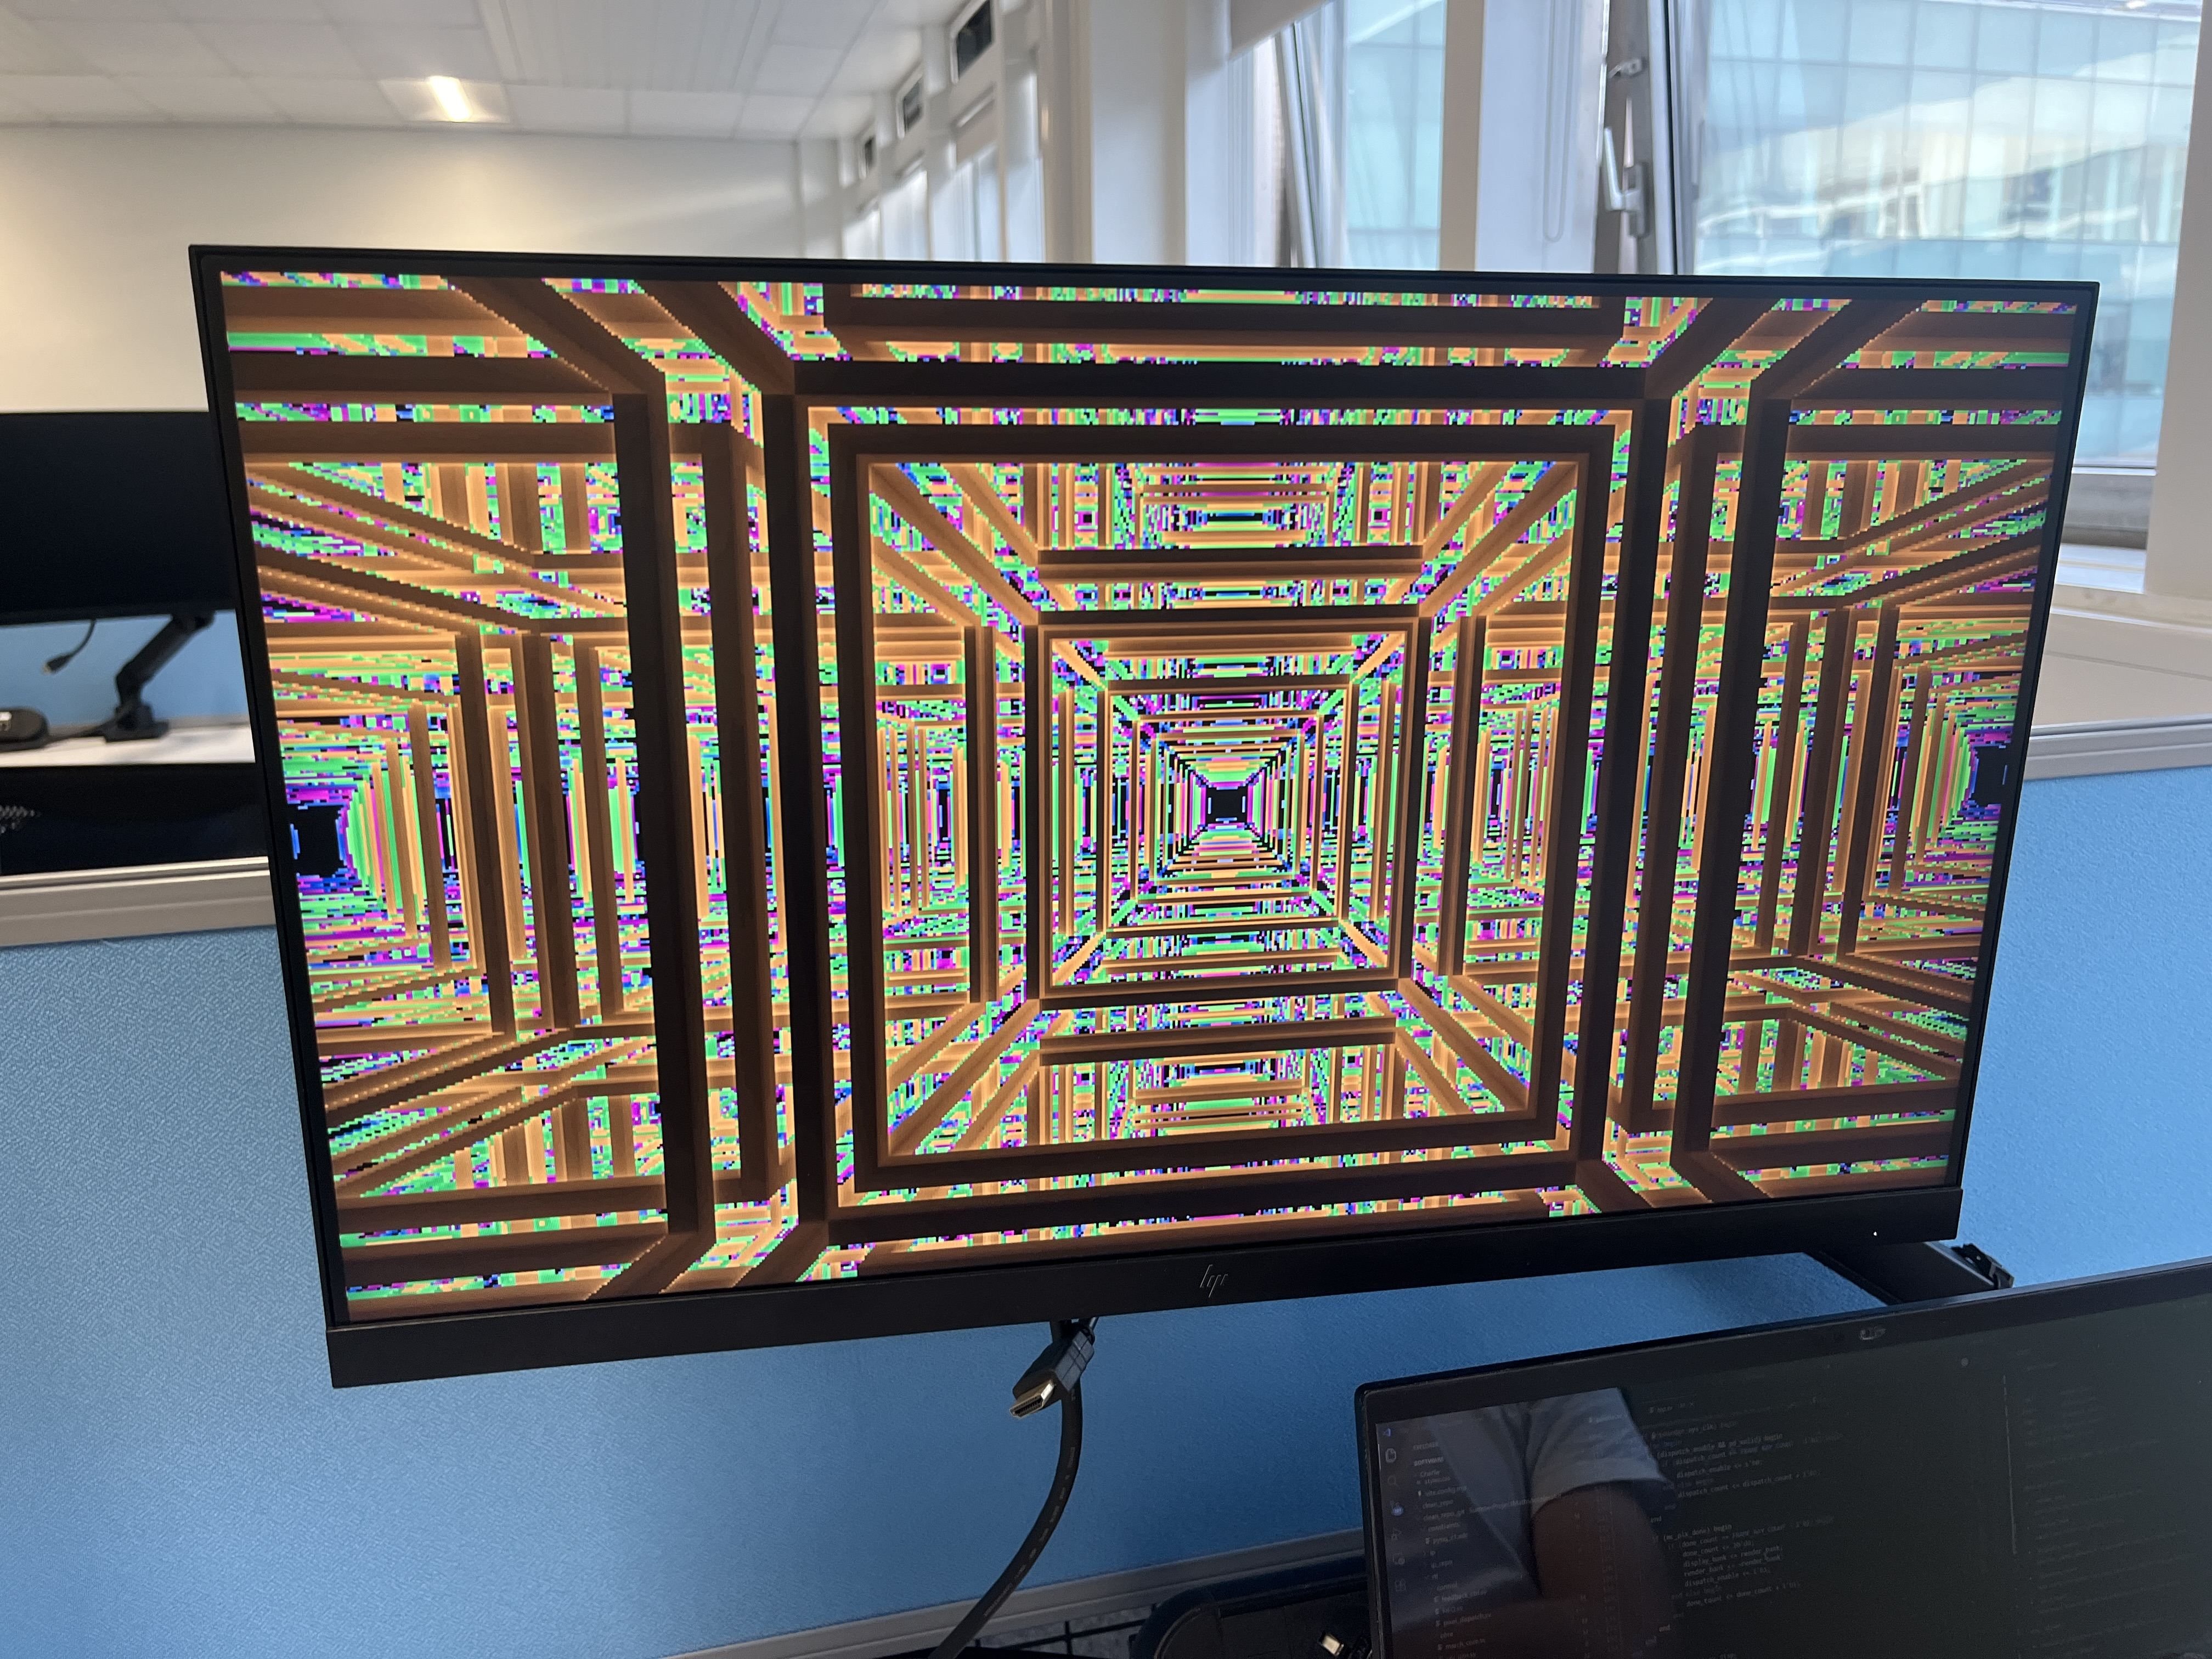
\includegraphics[width=\textwidth]{imgs/initial_scaffold.JPG}
        \vspace{-0.2cm}
        \captionof{figure}{First render of scaffold on screen, no split screen yet - no VR.}
        \label{fig:sphere_sdf_infinite}
    \end{minipage}%
    \hfill % Pushes the second minipage cleanly to the right margin
    \begin{minipage}{0.48\textwidth}
        \centering
        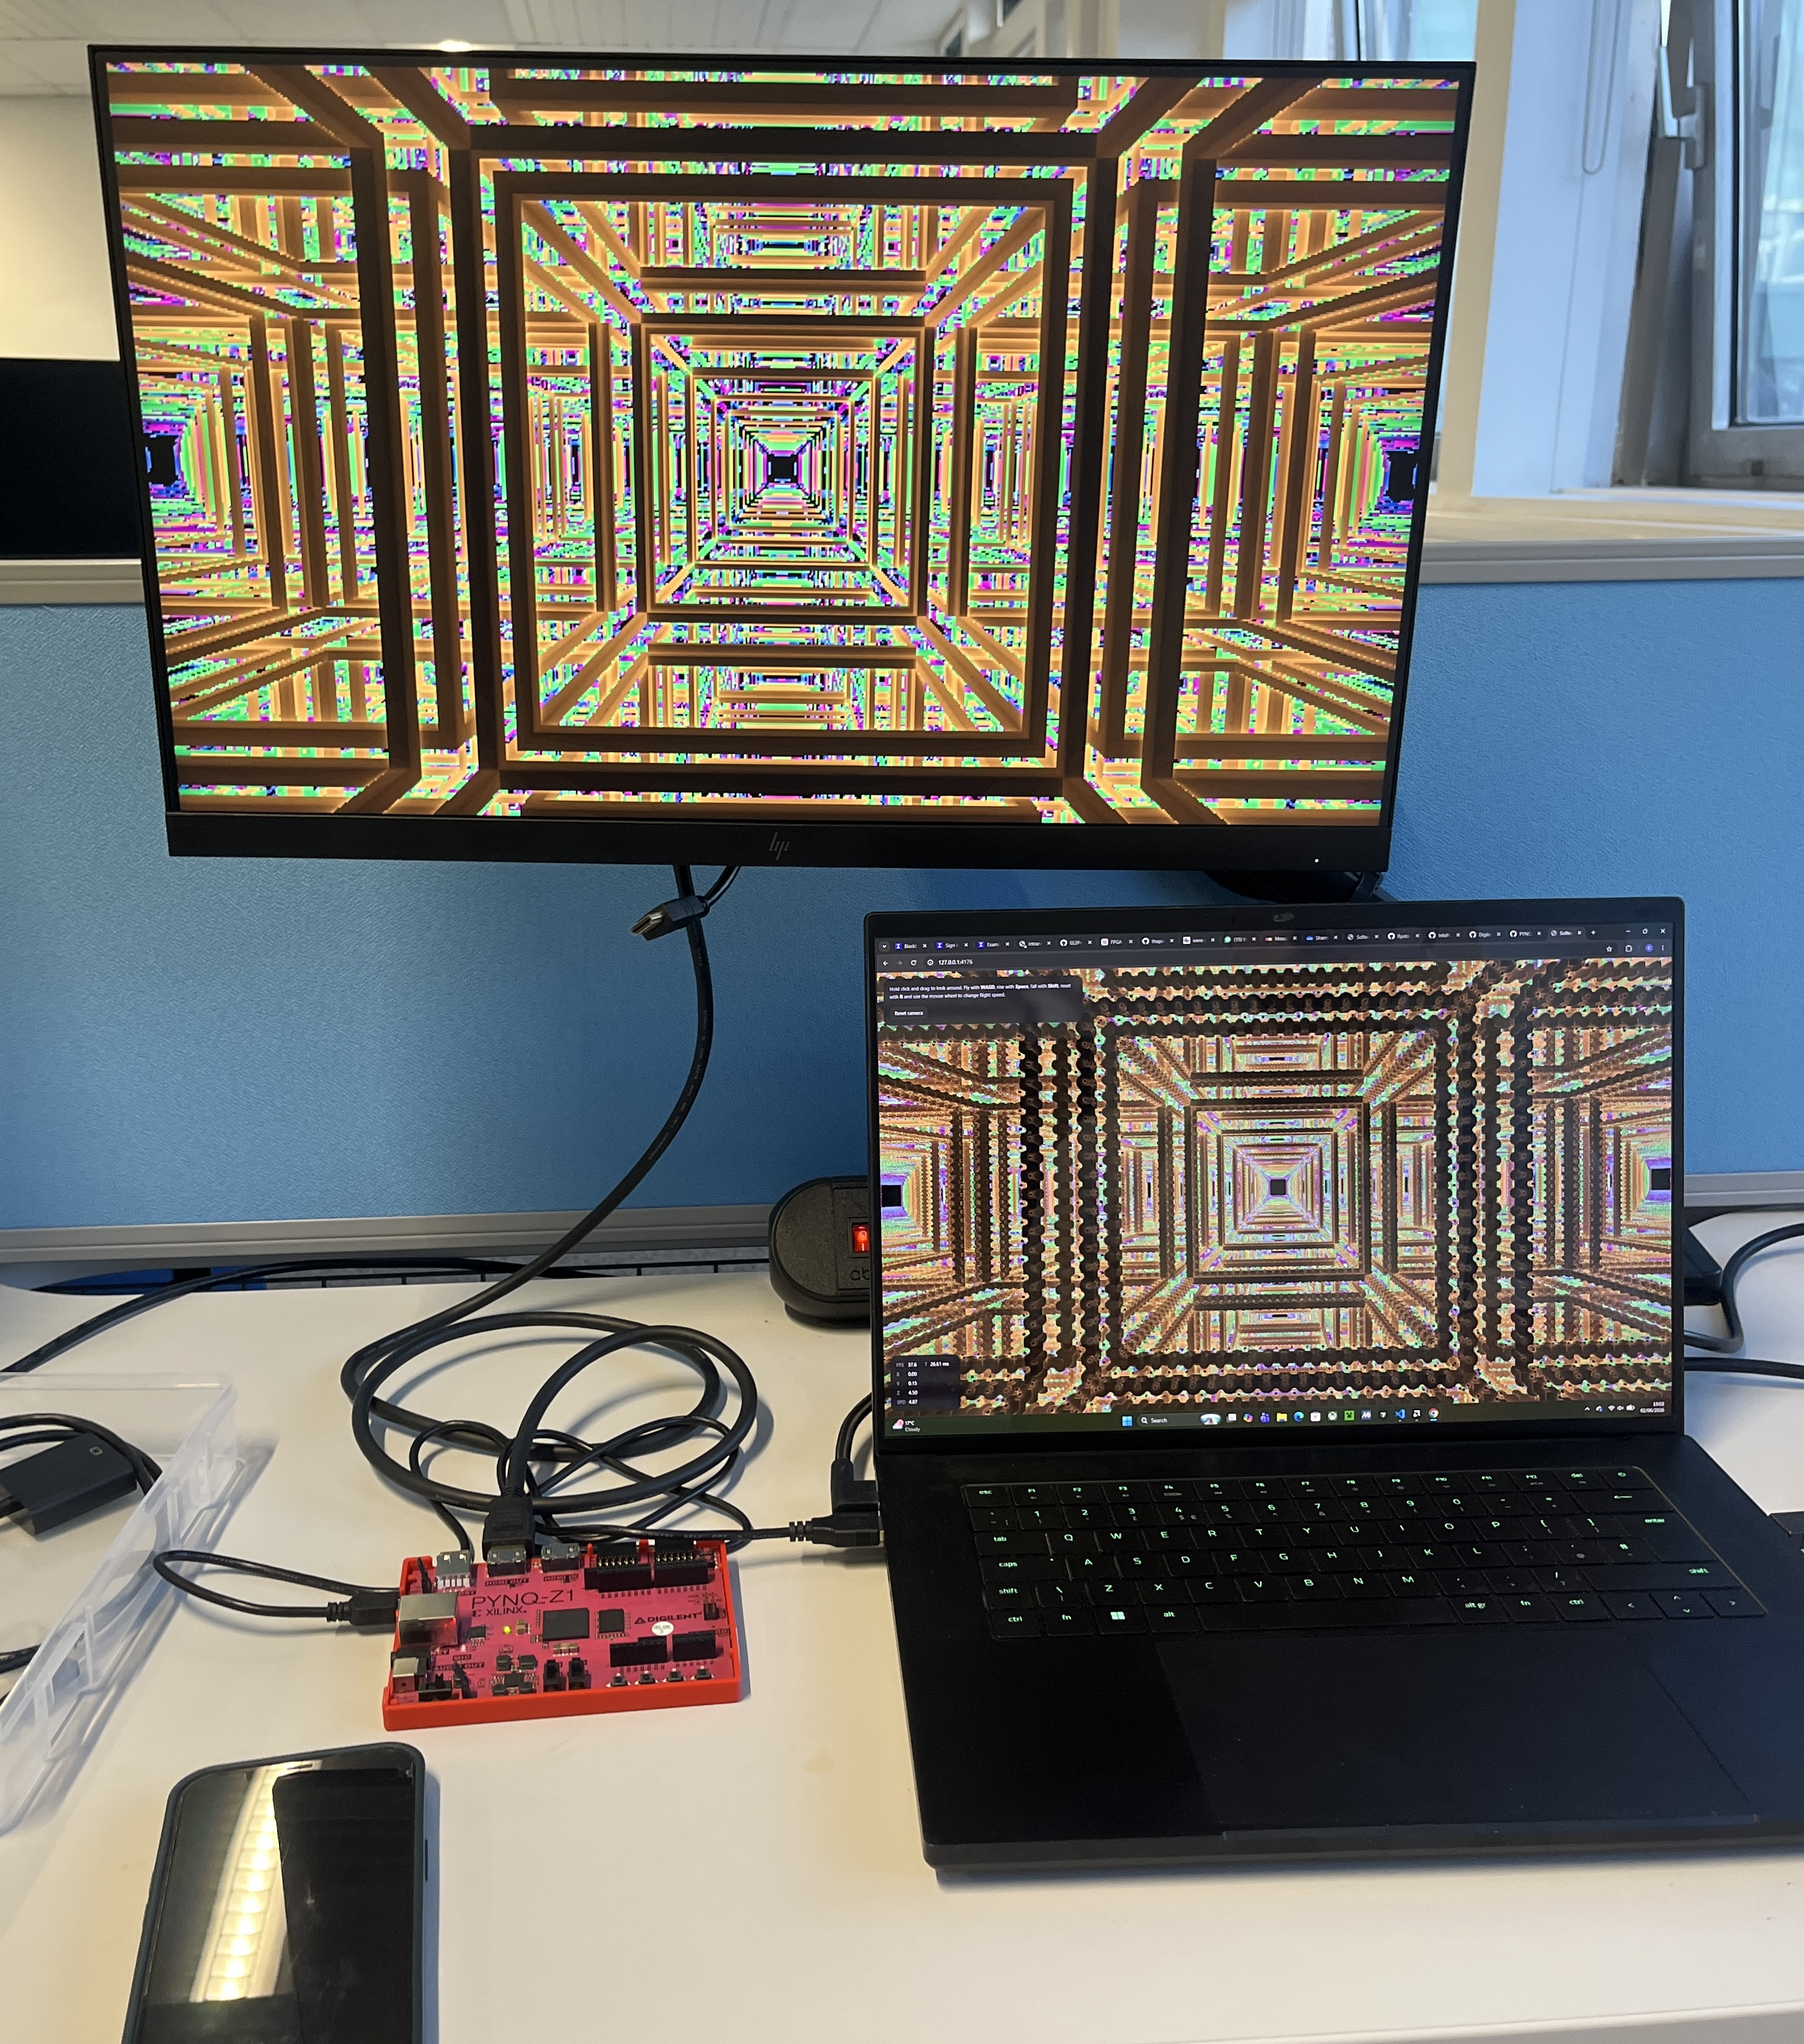
\includegraphics[width=\textwidth]{imgs/initial_scaffold2.jpg}
        \vspace{-0.2cm}
        \captionof{figure}{GSLS Version next to FPGA version, no movement yet}
        \label{fig:hardware_matrix_display}
    \end{minipage}
\end{center}
% ----------------------------------------------------------------

\subsection{Reciprocal and Division}

\paragraph{Reciprocal - \code{fp\_inverse.sv}.}
Newton-Raphson on $f(x) = 1/x - b$ gives $x_{n+1} = x_n(2 - bx_n)$, which
converges quadratically ($e_{n+1} = e_n^2$). The initial estimate flips the
exponent field, giving $bx_0 \in [1,2)$ and guaranteed convergence. Three
iterations of 12 cycles each reduce error from $\sim$25\% to $\sim$0.0015\%;
total latency: 36 cycles.

\paragraph{Division - \code{fp\_division.sv}.}
$a/b$ is computed as $a \times \text{fp\_inverse}(b)$, with $a$ delayed 36
cycles through \code{state\_pipe} to arrive cycle-aligned. Total latency: 40
cycles.

\subsection{Modulus - \code{fp\_modulus.sv}}

$a \bmod b = a - b\cdot\lfloor a/b\rfloor$, where \code{fp\_floor} is purely
combinational, masking fractional mantissa bits by exponent. The full chain -
division (40) $\to$ floor (0) $\to$ multiply (4) $\to$ subtract (4) - gives
52 cycles total, the most expensive primitive in the library and the dominant
term in SDF evaluation latency for space-repetition scenes.

\subsection{Pipeline Synchronisation - \code{state\_pipe}}

When two computation chains of unequal length must produce cycle-aligned
outputs, \code{state\_pipe} delays the shorter chain. It is a parameterised
shift register synthesised by Vivado as SRLs rather than flip-flop chains,
significantly reducing flip-flop usage. Misalignment by even one cycle produces
completely corrupted renders with no obvious visual diagnostic.

\subsection{Matrix-Vector Product - \code{fp\_mul\_vec3\_mat33.sv}}

Nine parallel \code{fp\_mul} instances compute all products of the $3\times3$
lookat matrix simultaneously in 4 cycles; three pairs of \code{fp\_add}
accumulate row sums in 4 more cycles. Total latency: 8 cycles, with no internal
synchronisation delay lines required, as all nine multiplies share the same
input register.

\FloatBarrier


% ===============================================================
\section{Ray Generation}
% ===============================================================

\subsection{Purpose and Design}
\code{ray\_gen.sv} is a fully pipeined, non-stalling module that converts pixel coordinates into world-space unit ray. It accepts one pixel per clock cycle  and produces the corresponding ray 45 cycles later.

\code{ray\_gen.sv} transforms a pixel coordinate $(p_x, p_y)$ and the camera
lookat matrix into a normalised world-space ray direction. The pixel coordinate
is first converted from screen space to normalised device coordinates (NDC),
scaled to a $[-1, 1]^2$ viewport, then transformed by the $3 \times 3$ lookat
matrix to produce the world-space direction. Coordinates are doubled
(working at $2\times$ integer resolution) to avoid non-integer pixel centres,
where the true centre of a $1280 \times 720$ display falls at $x = 639.5$,
represented exactly in $2\times$ space. The FOV is controlled by
\code{FOV\_Z\_CONST}, encoding the virtual focal length. At $1024\times600$ the
constant is set to \texttt{27'h221A000} ($\approx 83.3^\circ$ horizontal FOV). 

The conversion from integer pixel coordinates to FP27 is done by a fully
unrolled combinational function \code{fp\_int2fp} inside the module, avoiding
an extra pipeline stage.

Three SystemVerilog testbenches provide 47 tests with zero failures: \texttt{tb\_axi\_camera\_regs.sv} (16 tests, register write/readback and commit atomicity), \texttt{tb\_ray\_gen.sv} (17 tests, centre and off-axis pixel directions), and \texttt{tb\_fp\_ops.sv} (14 tests, FP27 arithmetic including $1/\sqrt{4.0} = 0.4991$, confirming Newton--Raphson convergence).

\subsection{AXI-Lite Camera Interface}

The PS communicates camera parameters to the PL through an AXI-Lite register
file at base address \texttt{0x43C00000}. The register map is:

\begin{table}[htbp]
\centering
\small
\caption{AXI-Lite camera register map}
\label{tab:axi_regs}
{\renewcommand{\arraystretch}{1.3}
\begin{tabular}{cll}
\toprule
\textbf{Register offset} & \textbf{Content} & \textbf{Width} \\
\midrule
\texttt{0x00}--\texttt{0x20} & Lookat matrix rows 0--8 & 9 $\times$ FP27 \\
\texttt{0x24}--\texttt{0x2C} & Camera origin $x, y, z$ & 3 $\times$ FP27 \\
\texttt{0x30}--\texttt{0x4C} & SDF parameters 0--7     & 8 $\times$ FP27 \\
\texttt{0x50} & Camera commit (write 1 to latch)       & 1-bit \\
\bottomrule
\end{tabular}}
\end{table}

\FloatBarrier

The commit register prevents the pipeline from reading a partially updated
camera matrix. The PS writes all 12 parameters then pulses the commit register,
atomically latching them into the registers visible to the PL.

\code{ray\_gen} has a fixed latency of 48 clock cycles, determined by the depth
of the \code{fp\_mul\_vec3\_mat33} chain (8 cycles) plus pipeline register stages
that prevent the module from becoming the critical path.


\FloatBarrier


% ===============================================================
\section{Ray Marcher Core}
\label{sec:marchcore}
% ===============================================================

\subsection{Architecture and Pipeline Stages}

\code{march\_core.sv} is the computational heart of the renderer. It receives
a pixel payload (coordinates, ray position, ray direction, iteration count,
accumulated distance) and performs one sphere-tracing step: evaluate the SDF
at the current position, advance the ray by the returned distance, and either
terminate the ray or return it to the feedback controller for another iteration.

The core is a three-stage fully pipelined architecture with per-iteration latency
of 163 clock cycles:

\begin{enumerate}
    \item \textbf{Ray generation (48 cycles).} On iteration 0, \code{ray\_gen}
    computes the world-space ray direction from the pixel coordinate and lookat
    matrix. On subsequent iterations this stage is bypassed --- the direction and
    position carried from the previous feedback output are used directly. A
    combinational mux selects between the two:
\begin{lstlisting}[language=Verilog]
localparam RG_LAT  = 48;
localparam SDF_LAT = 107;
localparam STEP_LAT = 8;

wire [26:0] s1_pos_x = (d1_iter == 8'd0) ? rg_orig[0] : d1_pos_x;
wire [26:0] s1_dir_x = (d1_iter == 8'd0) ? rg_dir[0]  : d1_dir_x;
\end{lstlisting}
    All feedback signals are delayed by exactly \texttt{RG\_LAT = 48} cycles
    using \code{state\_pipe} instances so they arrive at this mux simultaneously
    with the ray generation output.

    \item \textbf{SDF evaluation (107 cycles).} The current position
    $(p_x, p_y, p_z)$ is passed to the SDF module, which returns the signed
    distance to the nearest surface. For scenes using space repetition, the three
    FP modulus operations account for $3 \times 52$ cycles, but the modulus chains
    are partially parallel and the overall SDF latency for the scaffold scene is
    107 cycles. All position, direction, iteration count, and pixel ID signals
    are delayed through \code{state\_pipe} instances of depth 107 so they arrive
    cycle-aligned with the SDF output.

    \item \textbf{Step and hit detection (8 cycles).} The sphere-tracing step
    advances the ray position by the SDF distance:
    \[
        \mathbf{p}_{n+1} = \mathbf{p}_n + d_{\text{SDF}} \cdot \hat{\mathbf{r}}
    \]
    Three parallel \code{fp\_mul} instances compute $d \cdot r_x$, $d \cdot r_y$,
    $d \cdot r_z$, followed by three \code{fp\_add} instances, for 8 cycles total.
    Hit and miss conditions are evaluated combinationally:
\begin{lstlisting}[language=Verilog]
localparam [26:0] HIT_THRESH = {1'b0, 8'd117, 18'h01893}; // ~0.001
localparam        MAX_ITER   = 128;

wire hit_comb  = d3_valid & (d3_dist[26] | (d3_dist < HIT_THRESH));
wire miss_comb = d3_valid & (d3_iter >= MAX_ITER);
wire done_comb = hit_comb | miss_comb;
\end{lstlisting}

    \code{HIT\_THRESH} encodes $\approx 10^{-3}$: exponent field $117 = 127 - 10$
    gives $2^{-10}$; mantissa $\texttt{0x01893} \approx 0.024$; value
    $(1.024) \times 2^{-10} \approx 0.001$. A ray is also considered to have hit
    if the SDF returns a negative value (sign bit set), indicating the ray
    overshot the surface. \code{MAX\_ITER = 128} limits total depth; rays that
    never converge terminate and are coloured by their accumulated travel distance.
\end{enumerate}

Each cycle the core asserts either \code{pix\_done} (ray terminated; iteration count forwarded to the fog LUT for RGB mapping) or \code{fb\_valid} (ray continues; updated position and direction returned to \code{feedback\_ctrl}). Both paths are registered with no combinational output.

\subsection{Space Repetition in the Scaffold SDF}

The scaffold scene tiles infinite space by replacing the marched position with
its modulo equivalent in a canonical cell before SDF evaluation:

\begin{lstlisting}[language=Verilog]
assign cell_sz = sdf_params[0];  // bass FFT energy -> AXI-Lite reg
fp_modulus inst_x(.a(px), .b(cell_sz), .rem(rep_px));
fp_modulus inst_y(.a(py), .b(cell_sz), .rem(rep_py));
fp_modulus inst_z(.a(pz), .b(cell_sz), .rem(rep_pz));
\end{lstlisting}

\begin{figure}[h!]
\centering
\begin{tikzpicture}[
  arr/.style={-{Stealth[length=5pt]}, thick},
  cell/.style={draw=gray!60, fill=gray!10, minimum width=2cm, minimum height=2cm},
  canon/.style={draw=ImperialBlue, fill=blue!8, minimum width=2cm, minimum height=2cm, line width=1.2pt},
  obj/.style={circle, draw=red!70!black, fill=red!20, minimum size=0.55cm, inner sep=0pt},
  lbl/.style={font=\small},
]

%% --- tiling cells along x ---
\foreach \i/\col in {0/gray!10, 1/gray!10, 2/blue!8, 3/gray!10, 4/gray!10} {
  \pgfmathsetmacro\xi{\i*2.2}
  \draw[draw=gray!60, fill=\col, line width={\i==2 ? 1.2pt : 0.6pt}]
    (\xi, 0) rectangle ++(2.0, 2.0);
  % object ghost in each cell
  \node[obj, opacity={\i==2 ? 1 : 0.25}] at (\xi+1.0, 1.0) {};
}

%% canonical cell label
\node[font=\small\bfseries, color=ImperialBlue] at (2*2.2+1.0, 2.35) {canonical cell};

%% cell_sz brace
\draw[decorate, decoration={brace, amplitude=4pt, mirror}]
  (0, -0.25) -- (2.0, -0.25) node[midway, below=-15pt, font=\scriptsize] {\texttt{cell\_sz}};

%% camera
\node[draw, fill=yellow!20, minimum width=0.7cm, minimum height=0.5cm, font=\scriptsize] (cam) at (-1.8, 0.6) {cam};

%% ray line from camera across cells, hitting obj in cell 2
\draw[arr, color=black!70, dashed] (cam.east) -- (2*2.2+1.0, 1.0);

%% sample points on the ray
\foreach \xi/\yi in {0.5/0.72, 1.3/0.82, 2.8/0.90, 4.5/0.97} {
  \fill[black!50] (\xi, \yi) circle (1.8pt);
}

%% fmod arrow from sample in cell 0 down to canonical
\draw[arr, color=ImperialBlue, bend right=20]
  (0.5, 0.72) to node[lbl, left, xshift=-2pt]{\texttt{fmod(p,c)}} (2*2.2+0.5, 0.72);

%% hit annotation
\node[font=\scriptsize, color=red!70!black] at (2*2.2+1.0, 0.55) {SDF $<$ thresh};
\draw[-{Stealth[length=4pt]}, red!70!black] (2*2.2+1.0, 0.65) -- (2*2.2+1.0+0.25, 0.88);

%% miss annotation (cell 0)
\node[font=\scriptsize, color=black!50, align=center] at (1.0, -0.55) {SDF $\gg$ 0\\(step forward)};

\end{tikzpicture}
\caption{Space repetition via \texttt{fp\_modulus}: the ray position $\mathbf{p}$ at each march step is wrapped into the canonical cell by \texttt{fmod(p, cell\_sz)} before SDF evaluation. The infinite tiling is implicit - only one cell's SDF is ever evaluated. Bass FFT energy sets \texttt{cell\_sz} at runtime, expanding or compressing the tile density, effectively compressing and dilating space.}
\label{fig:space-rep}
\end{figure}

The key insight is that the SDF of an infinite tiling equals the SDF of a single
canonical cell evaluated at the wrapped coordinate. This is valid provided the
cell half-width exceeds the geometry's maximum extent. The cell size is written
from the PS each audio block, making the tiling density a live parameter driven
by bass energy. The \code{fp\_modulus} latency of 52 cycles dominates SDF
evaluation and drives the \code{SDF\_LAT = 107} parameter in \code{march\_core}.
Note that it is important to leave a spacing of minimum 0.1 units between cell size and object size/radius, as the Newton Raphson iterations for modulo, by nature inexact, can cause imprecisions and at worst bleeding (ie, geometry is lost as coloring no longer corresponds to due cell).

Space repetition tooks days to implement. The Newton Raphson logic is not easy and floor function in FP27 is quite difficult to understand (though basic in bit masking technique). Before infinite tiling, a Look Up Table approach was used to determine canonical positions at certain points. This caused the world to have borders, leading to interesting landscapes, see below!
\begin{figure}[htbp]
    \centering
    \begin{minipage}[b]{0.48\textwidth}
        \centering
        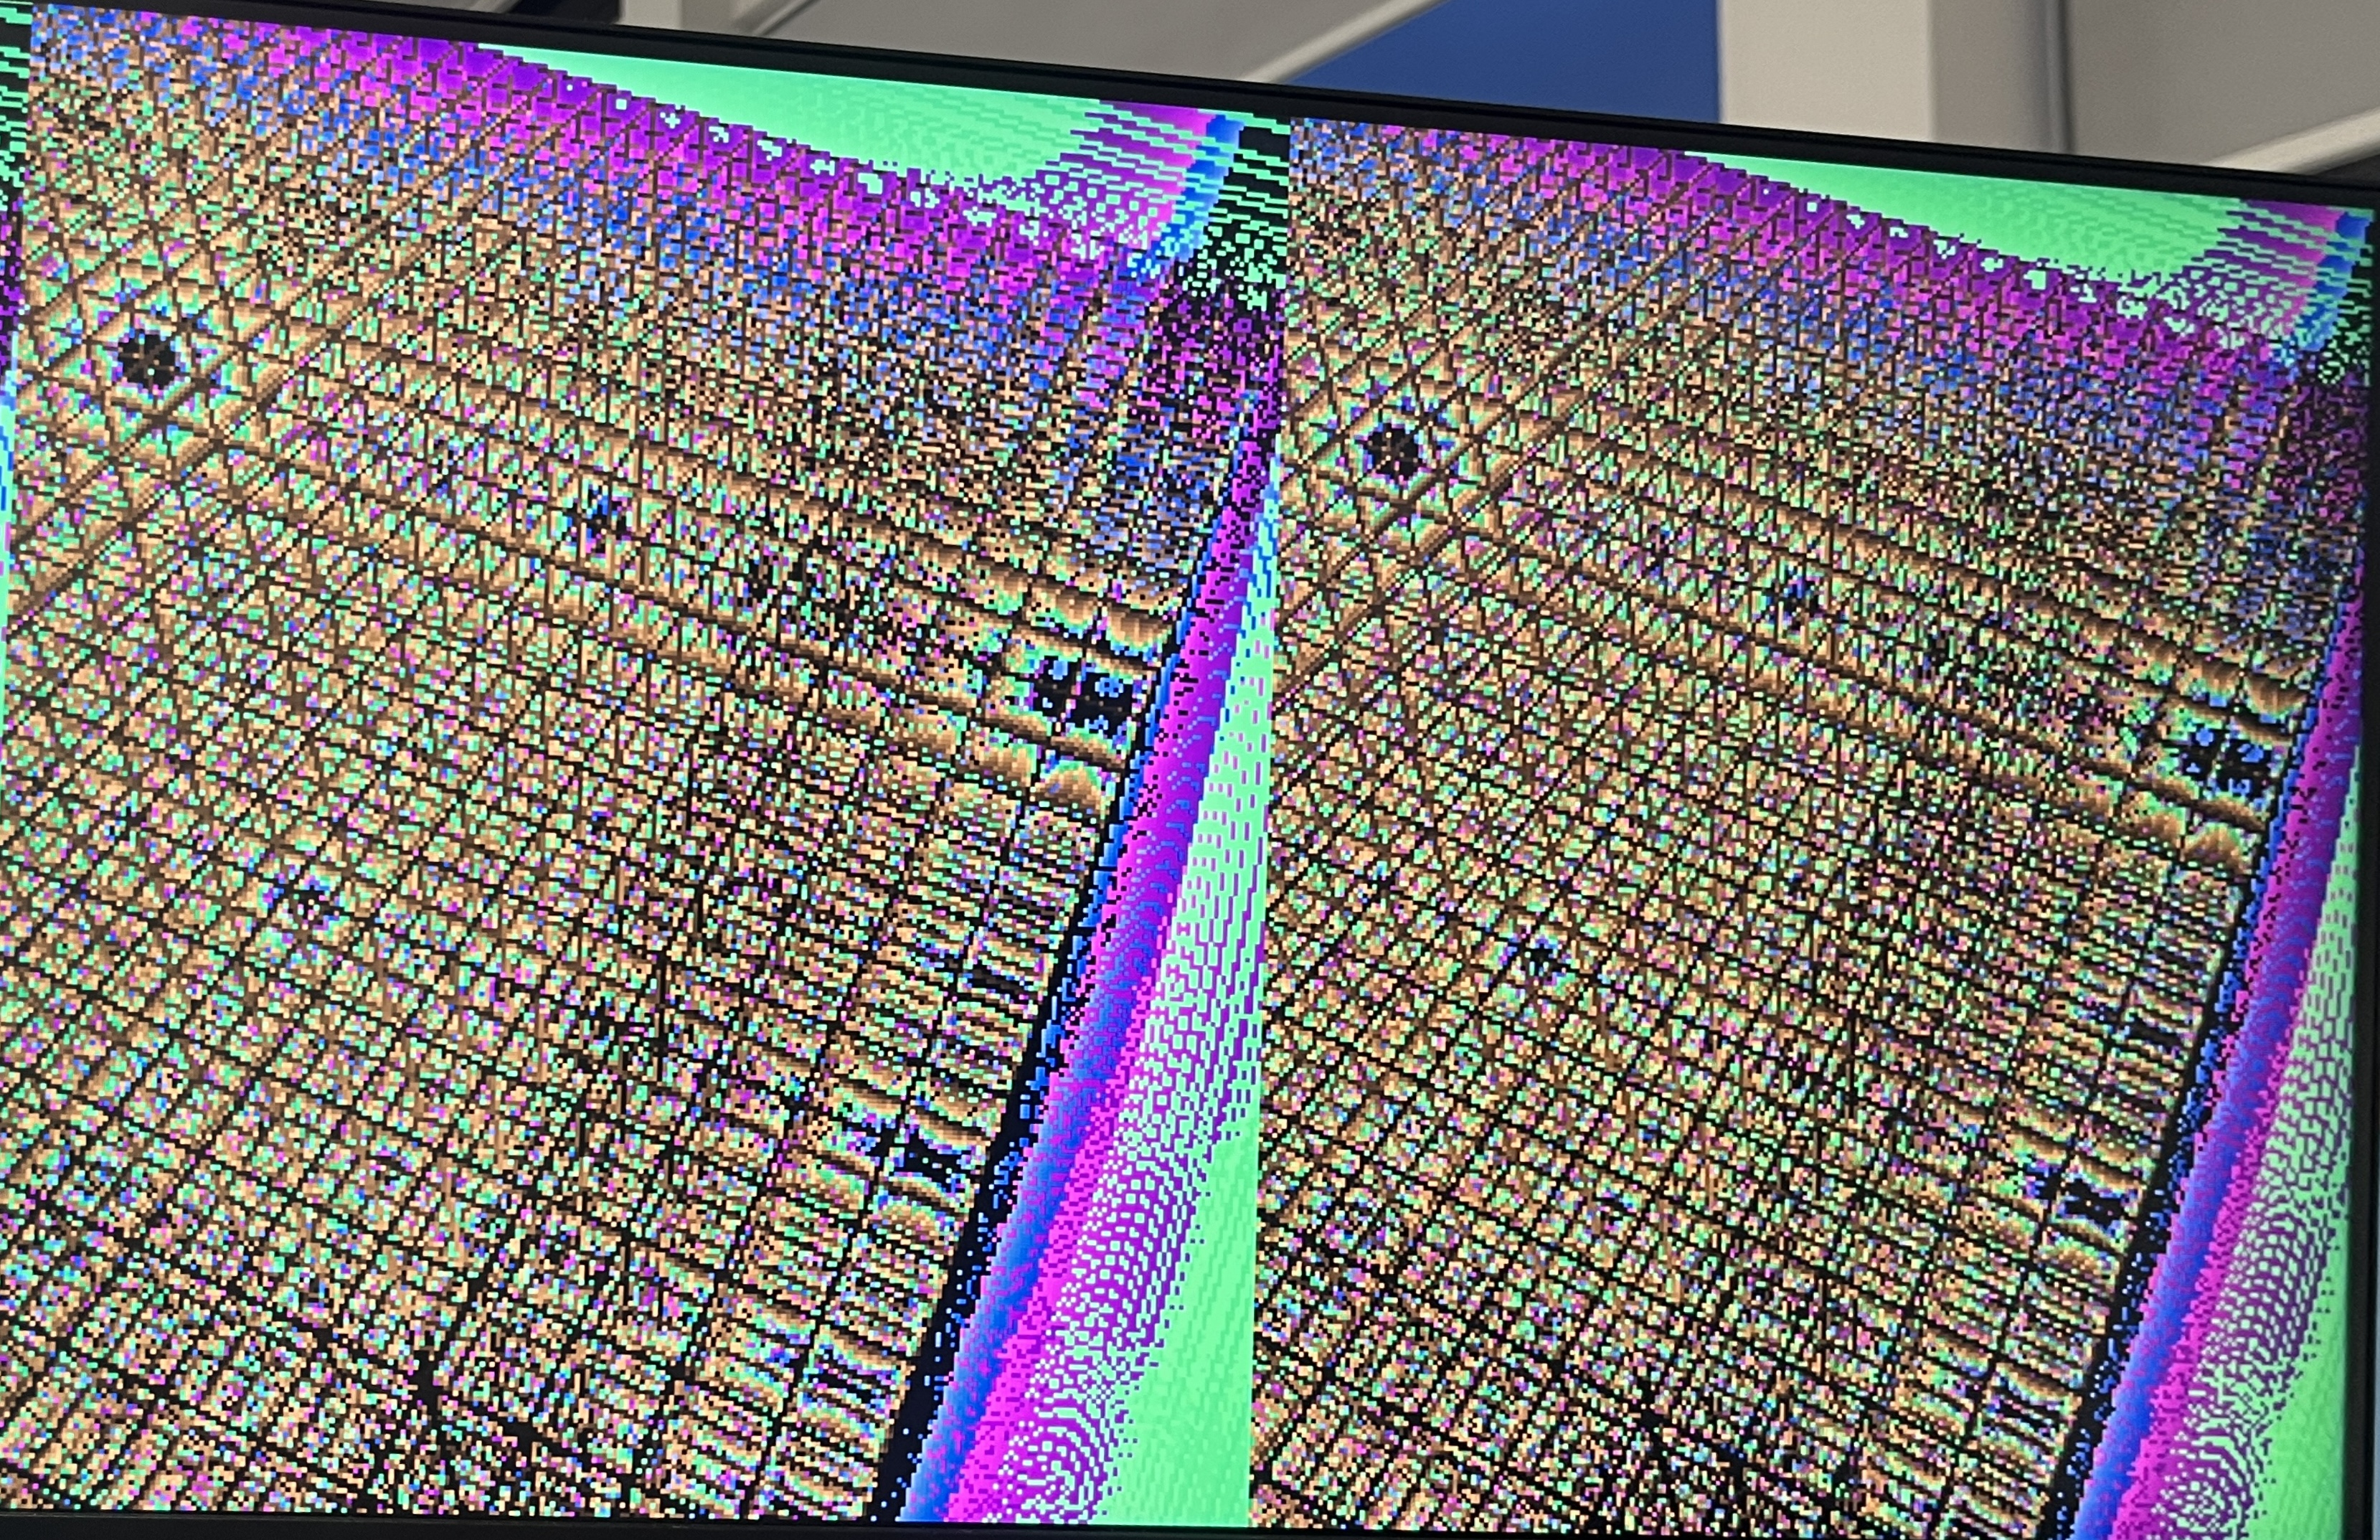
\includegraphics[width=\textwidth]{imgs/scaffold_borders1.jpg}
        \label{fig:image1}
    \end{minipage}
    \hfill
    \begin{minipage}[b]{0.48\textwidth}
        \centering
        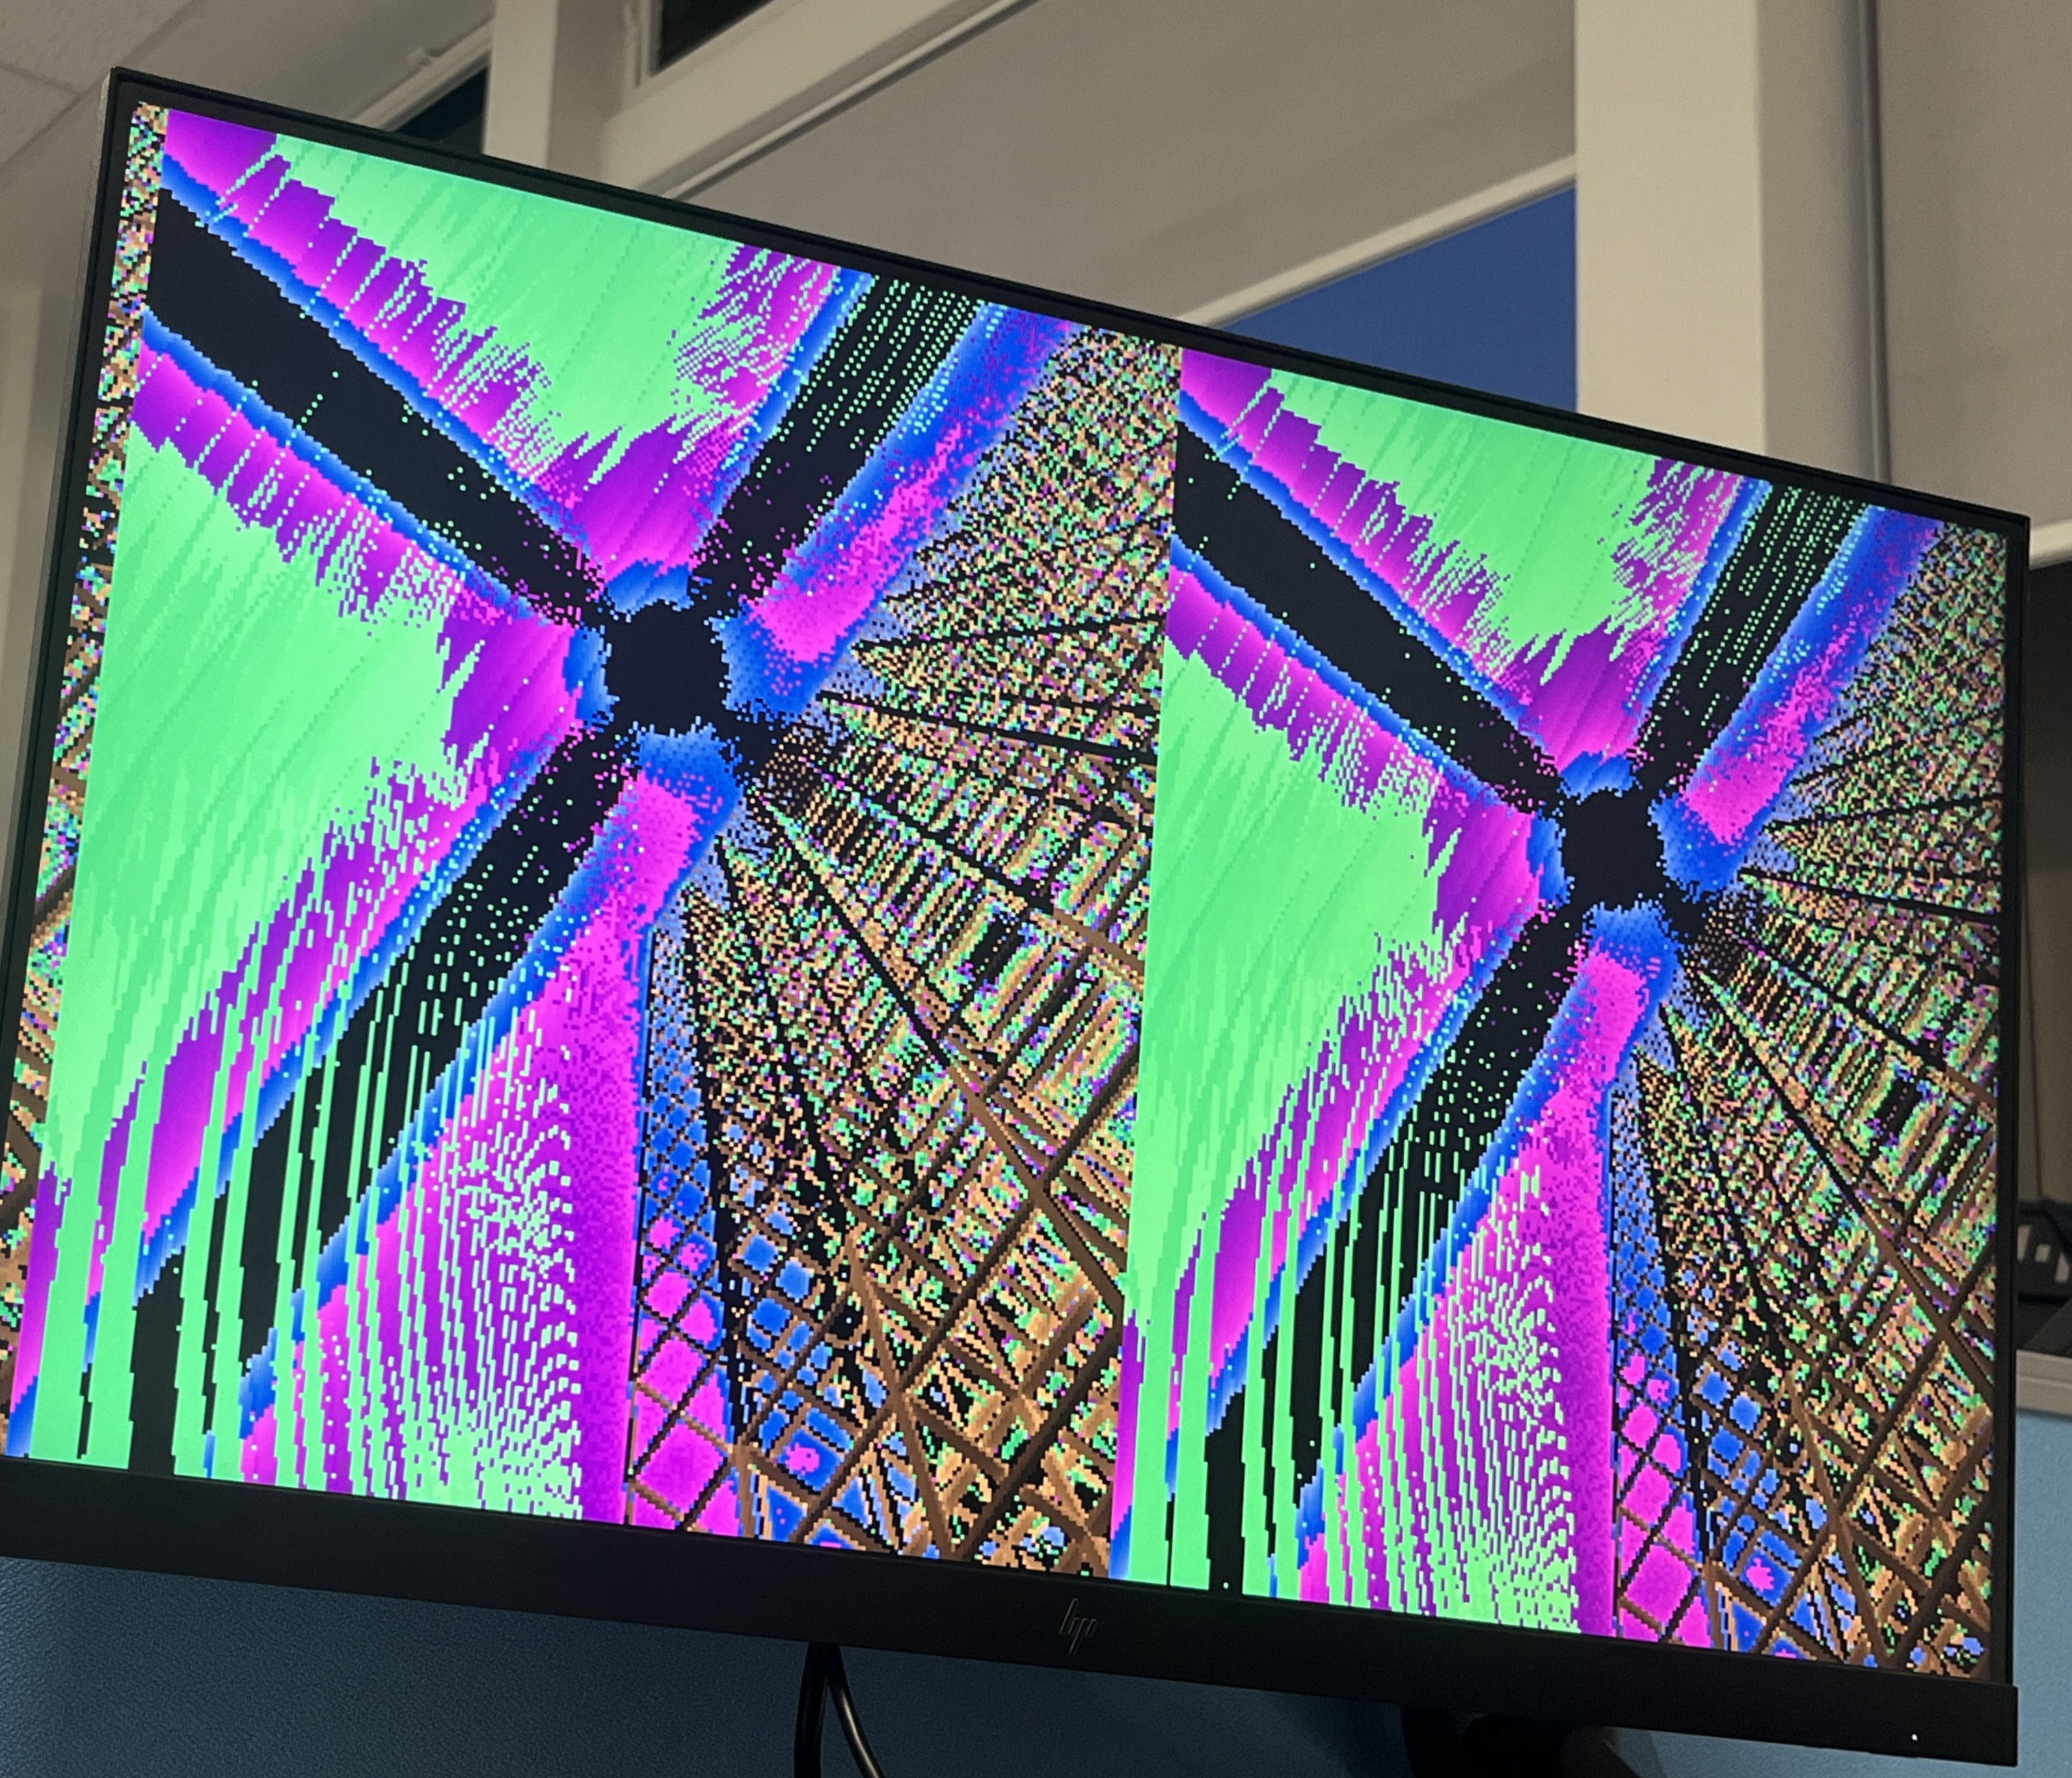
\includegraphics[width=\textwidth]{imgs/scaffold_borders2.jpg}
        \label{fig:image1000}
    \end{minipage}
    \caption{World edges visible, scaffold signed distance repetition suddenly stops.
    The exterior colouring is due to the periodic nature of palette.sv coloring.}
\end{figure}

\FloatBarrier


% ===============================================================
\section{Pixel Dispatch and Feedback Scheduling}
% ===============================================================

\subsection{Introduction}

The pixel pipelining comprises several hardware components ranging from initial
ray generation to final HDMI output. To ensure a controlled and ordered flow of
pixels, the infrastructure relies upon a coordinated traffic management layer.

\subsection{\code{pixel\_dispatch.sv}}

The first and most crucial component is \code{pixel\_dispatch}, which executes a
continuous raster scan of all on-screen pixels to guarantee deterministic
throughput. In addition to the coordinate stream, this module assigns a tracking
index (\code{pix\_id}) to each payload. The tag travels through the pipeline with
the ray data and allows downstream modules to map returning pixels to their
specific memory slots without losing coordinate context.

Once a valid pixel is obtained from the raster scan, \code{pixel\_dispatch}
samples the synchronous \code{pipeline\_ready} signal asserted by
\code{feedback\_ctrl}. A high signal invites the dispatcher to advance its
raster count and stream Cartesian coordinates and the 20-bit pixel ID to the
ray generation module. A low signal indicates the feedback loop is under
execution; \code{pixel\_dispatch} applies backpressure by stalling its counter,
preventing FIFO overflow and protecting the feedback loop against structural
deadlock.

\subsection{\code{feedback\_ctrl.sv}}

\code{feedback\_ctrl} arbitrates between new coordinates from
\code{pixel\_dispatch} and active rays returning from the march core, mirroring
a multiplexer. Since the ray generator and march core are deep pipelined
architectures, many pixels are simultaneously in-flight. Rays requiring
additional iterations must be routed back to the front of the pipeline via a
FIFO storage buffer.

When the FIFO is non-empty, \code{feedback\_ctrl} asserts \code{read\_enable},
passes the stored payload to the ray generator, and sends a backpressure signal
to \code{pixel\_dispatch} to stall the raster counter. When the FIFO is empty,
\code{pixel\_dispatch} advances and a new pixel enters the pipeline directly.
The feedback loop is always prioritised to prevent structural deadlock.

\subsection{\code{FIFO.sv}}

\code{FIFO.sv} implements a synchronous dual-port memory array with read and
write pointers. The payload width was carefully compressed to 190 bits per entry.
Numerical analysis of the pipeline gives a maximum in-flight pixel count of 103
cycles (48 ray gen + 55 march). A 128-entry deep FIFO provides 24.3\% headroom,
accommodating transient stalls without interfering with active pixels.

\subsection{\code{fb\_write.sv}}

\code{fb\_write} extracts the iteration count from completed rays, raises
\code{bram\_we}, and maps the \code{pix\_id} to the correct framebuffer address.
The framebuffer is a dual-port BRAM: one port handles write operations from
\code{fb\_write}, the other is dedicated to HDMI scan-out, bridging the rendering
and pixel clock domains without metastability.

\subsection{Verification}

\begin{table}[htbp]
\centering
\small
\caption{Pixel management verification results}
\label{tab:pixel_verification}
{\renewcommand{\arraystretch}{1.3}
\begin{tabular}{llp{6.5cm}}
\toprule
\textbf{Testbench} & \textbf{Module} & \textbf{Result} \\
\midrule
\code{pixel\_dispatch\_tb.sv} & \code{pixel\_dispatch} & PASS: all 921,600 pixels emitted exactly once \\
\code{feedback\_ctrl\_tb.sv}  & \code{feedback\_ctrl}  & PASS: FIFO stall and priority arbitration correct \\
\code{fb\_write\_tb.sv}       & \code{fb\_write}       & PASS: \code{bram\_we} and address on every done pixel \\
\code{integration\_tb.sv}     & Full interface         & PASS: $640\times360$ screen with zero duplicates \\
\bottomrule
\end{tabular}}
\end{table}

\FloatBarrier

\section{Timing Closure: 40Mhz to 200Mhz}

  The initial design ran at 40\,MHz with WNS\,=\,$+$16.3\,ns. Reaching                                                      
  200\,MHz required ten iterations of identifying and breaking critical paths
  from post-route timing reports:                                                                                           
                  
  \begin{itemize}
    \item \textbf{fp\_add casex priority encoder:} The stage-4 leading-one
    scan synthesised to a ripple chain of $\sim$20 LUT levels ($\sim$8\,ns).
    Replacing it with a flat \texttt{casex} enumerating all 20 shift amounts
    reduced the depth to $\sim$5 LUT levels.

    \item \textbf{fp\_mul DSP targeting and register insertion:} The
    19$\times$19 mantissa multiply used one DSP48E1 plus a 6-level fabric
    carry chain (5.7\,ns). Adding \texttt{(* use\_dsp = "yes" *)} eliminated
    the fabric path entirely, reducing delay to 1.9\,ns.

    \item \textbf{Pipeline register insertions:} Cascaded \texttt{fp\_min}
    comparators in \texttt{scene\_sdf} formed an 11-level, 7.1\,ns path;
    a register inserted between them halved the depth (\texttt{SDF\_LAT}
    incremented by 1 to compensate).

    \item \textbf{FIFO depth reduction and XDC constraints:} The DDR write
    FIFO at \texttt{FIFO\_DEPTH\,=\,4096} required 2880 RAM64E cells spanning
    34 fabric columns (WNS\,=\,$-$0.312\,ns). Reducing depth to 1024 collapsed
    the 64:1 mux to 16:1, cutting routing delay to 0.7\,ns. A pblock
    (\texttt{SLICE\_X0Y0:SLICE\_X69Y149}) confined \texttt{march\_core} to a
    contiguous region, and \texttt{(* max\_fanout\,=\,16 *)} was applied to
    the write-enable bus.

    \item \textbf{Pipeline resynchronisation:} When \texttt{fp\_mul} grew from
    3 to 4 cycles and \texttt{fp\_isqrt} from 10 to 16 cycles, flashing
    artefacts appeared on hardware. The root cause was \texttt{march\_core}
    pairing the SDF distance evaluated for ray $N$ with the position of ray
    $N+4$. All companion \texttt{state\_pipe} depths were recalculated to
    restore exact alignment.
  \end{itemize}

  The final 200\,MHz implementation reports WNS\,=\,0.000\,ns,
  TNS\,=\,0.000\,ns, and 0 failing endpoints.

  \begin{table}[h!]
  \centering
  \caption{Timing at each frequency milestone}
  \begin{tabular}{lrrrr}
  \hline
  \textbf{Milestone} & \textbf{Freq} & \textbf{Period} & \textbf{WNS} & \textbf{Failing} \\
  \hline
  Baseline (bring-up fixes) & 40\,MHz  & 25.0\,ns & $+$16.300\,ns & 0 \\
  Milestone 1               & 100\,MHz & 10.0\,ns & $+$0.067\,ns  & 0 \\
  Milestone 2               & 150\,MHz &  6.7\,ns & $+$0.145\,ns  & 0 \\
  Milestone 3               & 200\,MHz &  5.0\,ns & $+$0.000\,ns  & 0 \\
  \hline
  \end{tabular}
  \end{table}

  \begin{table}[h!]
  \centering
  \caption{150\,MHz iterative closure}
  \begin{tabular}{lrrr}
  \hline
  \textbf{Change applied} & \textbf{WNS (ns)} & \textbf{TNS (ns)} & \textbf{Failing} \\
  \hline
  Initial 150\,MHz                     & $-$2.514 & $-$2243   & 2385 \\
  fp\_add casex + parallel subtractors & $-$1.738 & $-$1125   & 1983 \\
  Pblock + impl strategy               & $-$0.681 & $-$173    &  614 \\
  scene\_sdf pipeline register         & $-$0.629 & $-$1098   &  120 \\
  fp\_mul stage split + DSP forcing    & $-$0.364 & $-$196    &   90 \\
  sdf\_term pipeline register          & $+$0.100 &     0     &    0 \\
  Resync (PIPE/RG/SDF\_LAT)           & $-$0.062 & $-$0.265  &    7 \\
  BRAM write pipeline                  & $+$0.145 &     0     &    0 \\
  \hline
  \end{tabular}
  \end{table}

  \begin{table}[h!]
  \centering
  \caption{200\,MHz violation fixes}
  \begin{tabular}{llr}
  \hline
  \textbf{Change} & \textbf{Description} & \textbf{Violation} \\
  \hline
  Deep pipeline + resync      & fp\_add/mul $4\to5$\,cy, isqrt $16\to20$\,cy  & $-$2.100\,ns \\
  max\_fanout=16 BRAM ctrl    & FF replication across 140 BRAMs                & $-$0.096\,ns \\
  AREG/BREG absorption fix    & Removed conflicting max\_fanout=1 on DSP       & $-$0.012\,ns \\
  Barrel-shifter mask removal & Pure shift; 2 CARRY4 stages eliminated         & $-$0.017\,ns \\
  pixel\_dispatch revert      & Ghost-ray drop causing black screen; reverted   & functional   \\
  \textbf{Final}              &                                                & \textbf{0.000\,ns} \\
  \hline
  \end{tabular}
  \end{table}

  \begin{table}[h!]
  \centering
  \caption{Module latency evolution (cycles)}
  \begin{tabular}{lrrr}
  \hline
  \textbf{Module} & \textbf{100\,MHz} & \textbf{150\,MHz} & \textbf{200\,MHz} \\
  \hline
  fp\_mul    &  2 &  4 &  5 \\
  fp\_add    &  4 &  4 &  5 \\
  fp\_isqrt  & 10 & 16 & 20 \\
  fp\_length & 10 & 32 & 40 \\
  ray\_gen   & 35 & 48 & 60 \\
  scene\_sdf & 44 & 55 & 69 \\
  \hline
  \end{tabular}
  \end{table}
% ===============================================================
\section{Signed Distance Field: Analytic Scenes}
% ===============================================================

\subsection{Purpose and Design}

The ray marcher accepts a scene selection input which allows the system to
substitute different SDF modules without modifying the march core pipeline.
A uniform module interface is used across all scenes: inputs are \code{clk},
\code{px}, \code{py}, \code{pz}, \code{sdf\_params[0:7]}, and the output is
always \code{sdf\_out [26:0]}. This uniform structure allows simple substitution
into \code{march\_core}; each scene is compiled as its own bitstream.

An SDF returns the exact shortest distance from a point $\mathbf{p}$ to the
boundary of a shape. Negative values indicate interior points. All modules use
the custom FP27 library; constants such as radii are encoded as 27-bit
\code{localparams} with explicit sign, exponent, and mantissa fields.

\subsection{Researched Shapes}

\begin{table}[htbp]
\centering
\small
\caption{SDF shape library}
\label{tab:sdf_library}
{\renewcommand{\arraystretch}{1.2}
\begin{tabular}{llc}
\toprule
\textbf{Module} & \textbf{SDF Formula} & \textbf{Latency (cycles)} \\
\midrule
\code{sdf\_sphere}         & $d = \|\mathbf{p}\| - r$                                         & ${\sim}13$ \\
\code{sdf\_torus}          & $d = \sqrt{(\sqrt{x^2+z^2}-R)^2+y^2} - r$                      & ${\sim}21$ \\
\code{sdf\_twisted\_torus} & Torus with height-dependent $XZ$ rotation                        & ${\sim}36$ \\
\code{sdf\_gyroid}         & $d \approx (\sin x\cos y + \sin y\cos z + \sin z\cos x)/4$     & ${\sim}28$ \\
\code{sdf\_octahedron}     & $d = (|x|+|y|+|z|-s)/\sqrt{3}$                                  & ${\sim}16$ \\
\code{sdf\_hyperboloid}    & $d = \sqrt{x^2+z^2} - \sqrt{(y/b)^2+1}$                         & ${\sim}20$ \\
\code{sdf\_star}           & Six-fold rotational fold + \code{sdf\_term}                      & ${\sim}20$ \\
\code{sdf\_box}            & \code{sdf\_term}$(|\mathbf{p}| - \mathbf{b})$                    & ${\sim}8$  \\
\code{sdf\_capsule}        & $d = \|\mathbf{p} - \text{clamp}(p_y)\hat{y}\| - r$            & ${\sim}8$  \\
\code{sdf\_mandelbulb}     & Power-8 Mandelbulb approximation                                 & ${\sim}12$ \\
\bottomrule
\end{tabular}}
\end{table}

\FloatBarrier                                                                                                             
                                                                                                                            
  \begin{table}[h]                                                                                                          
  \centering                                                                                                                
  \caption{Implemented signed distance functions: formulae, pipeline implementation, and latency}                           
  \label{tab:sdfs}
  \setlength{\arrayrulewidth}{0.4mm}
  \renewcommand{\arraystretch}{1.4}
  \begin{tabular}{|p{2.4cm}|p{4.2cm}|p{5.8cm}|p{2.0cm}|}
  \hline
  \textbf{SDF} & \textbf{Formula} & \textbf{Pipeline Implementation} & \textbf{Latency} \\
  \hline\hline

  \textbf{A: Sphere}
  &
  Unit sphere of radius $r$:
  $d = \|\mathbf{p}\| - r$
  &
  \texttt{fp\_length} computes the Euclidean norm; \texttt{fp\_sub} subtracts the radius in 4 cycles.
  &
  ${\sim}13$ cycles \\
  \hline

  \textbf{B: Torus}
  &
  Two radii: major $R$ (ring centre), minor $r$ (tube radius):
  $d = \sqrt{(\sqrt{x^2+z^2}-R)^2+y^2} - r$
  &
  The 3D problem reduces to 2D: the radial distance in the $XZ$ plane gives $q_x = \sqrt{x^2+z^2} - R$ (8 cycles). A
  \texttt{state\_pipe} of depth 8 aligns $q_y = p_y$ with $q_x$ before the second \texttt{fp\_length} and final subtraction.
  &
  ${\sim}21$ cycles \\
  \hline

  \textbf{C: Twisted Torus}
  &
  Height-dependent rotation applied to the $XZ$ plane before the torus SDF.
  &
  Both trigonometric functions are approximated via Taylor series valid for $|\theta| < \pi/4$. \texttt{TWIST = 0.25}
  ensures $\theta$ stays within the convergence region for all scene $p_y$ values.
  &
  ${\sim}36$ cycles \\
  \hline

  \textbf{D: Gyroid}
  &
  Infinite triply periodic minimal surface:
  $d \approx \tfrac{1}{4}(\sin x\cos y + \sin y\cos z + \sin z\cos x)$
  &
  Six Taylor-series approximations run in parallel; each cosine output is piped by 4 cycles to synchronise with its sine
  partner before multiplication.
  &
  ${\sim}28$ cycles \\
  \hline

  \textbf{E: Hyperboloid}
  &
  ---
  &
  Uses \texttt{fp\_isqrt} directly; its output is reciprocated to give $\sqrt{(y/b)^2+1}$ without a separate square root
  call.
  &
  \\
  \hline

  \textbf{F: Octahedron}
  &
  ---
  &
  Sums three absolute values and scales by $1/\sqrt{3}$ (encoded as a FP27 constant). A confirmed bug in the original
  constant (\texttt{18'h14888}, wrong) was corrected to \texttt{18'h09E6A}.
  &
  \\
  \hline

  \textbf{G: Star}
  &
  ---
  &
  Applies a six-fold rotational fold reducing computation to a single arm.
  &
  \\
  \hline

  \end{tabular}
  \end{table}

  \FloatBarrier

% ===============================================================
\section{Mandelbox}
% ===============================================================

\subsection{Introducing Mandelbox}

The Mandelbox is a 3D fractal defined by iterating a fold-and-scale map on a point
$\mathbf{v}$, generating complex geometry through geometric reflections and inversions rather than smooth polynomial escape conditions. Figure~\ref{fig:mandelbox-glsl} shows the GLSL reference render at 4.3\,fps on CPU.

\vspace{\fill} 
\begin{center}
    \nopagebreak % Strictly prevents a page break right before the image block
    \begin{minipage}{0.4\textwidth} % Slightly downscaled width from 0.85 to open up vertical budget
        \centering
        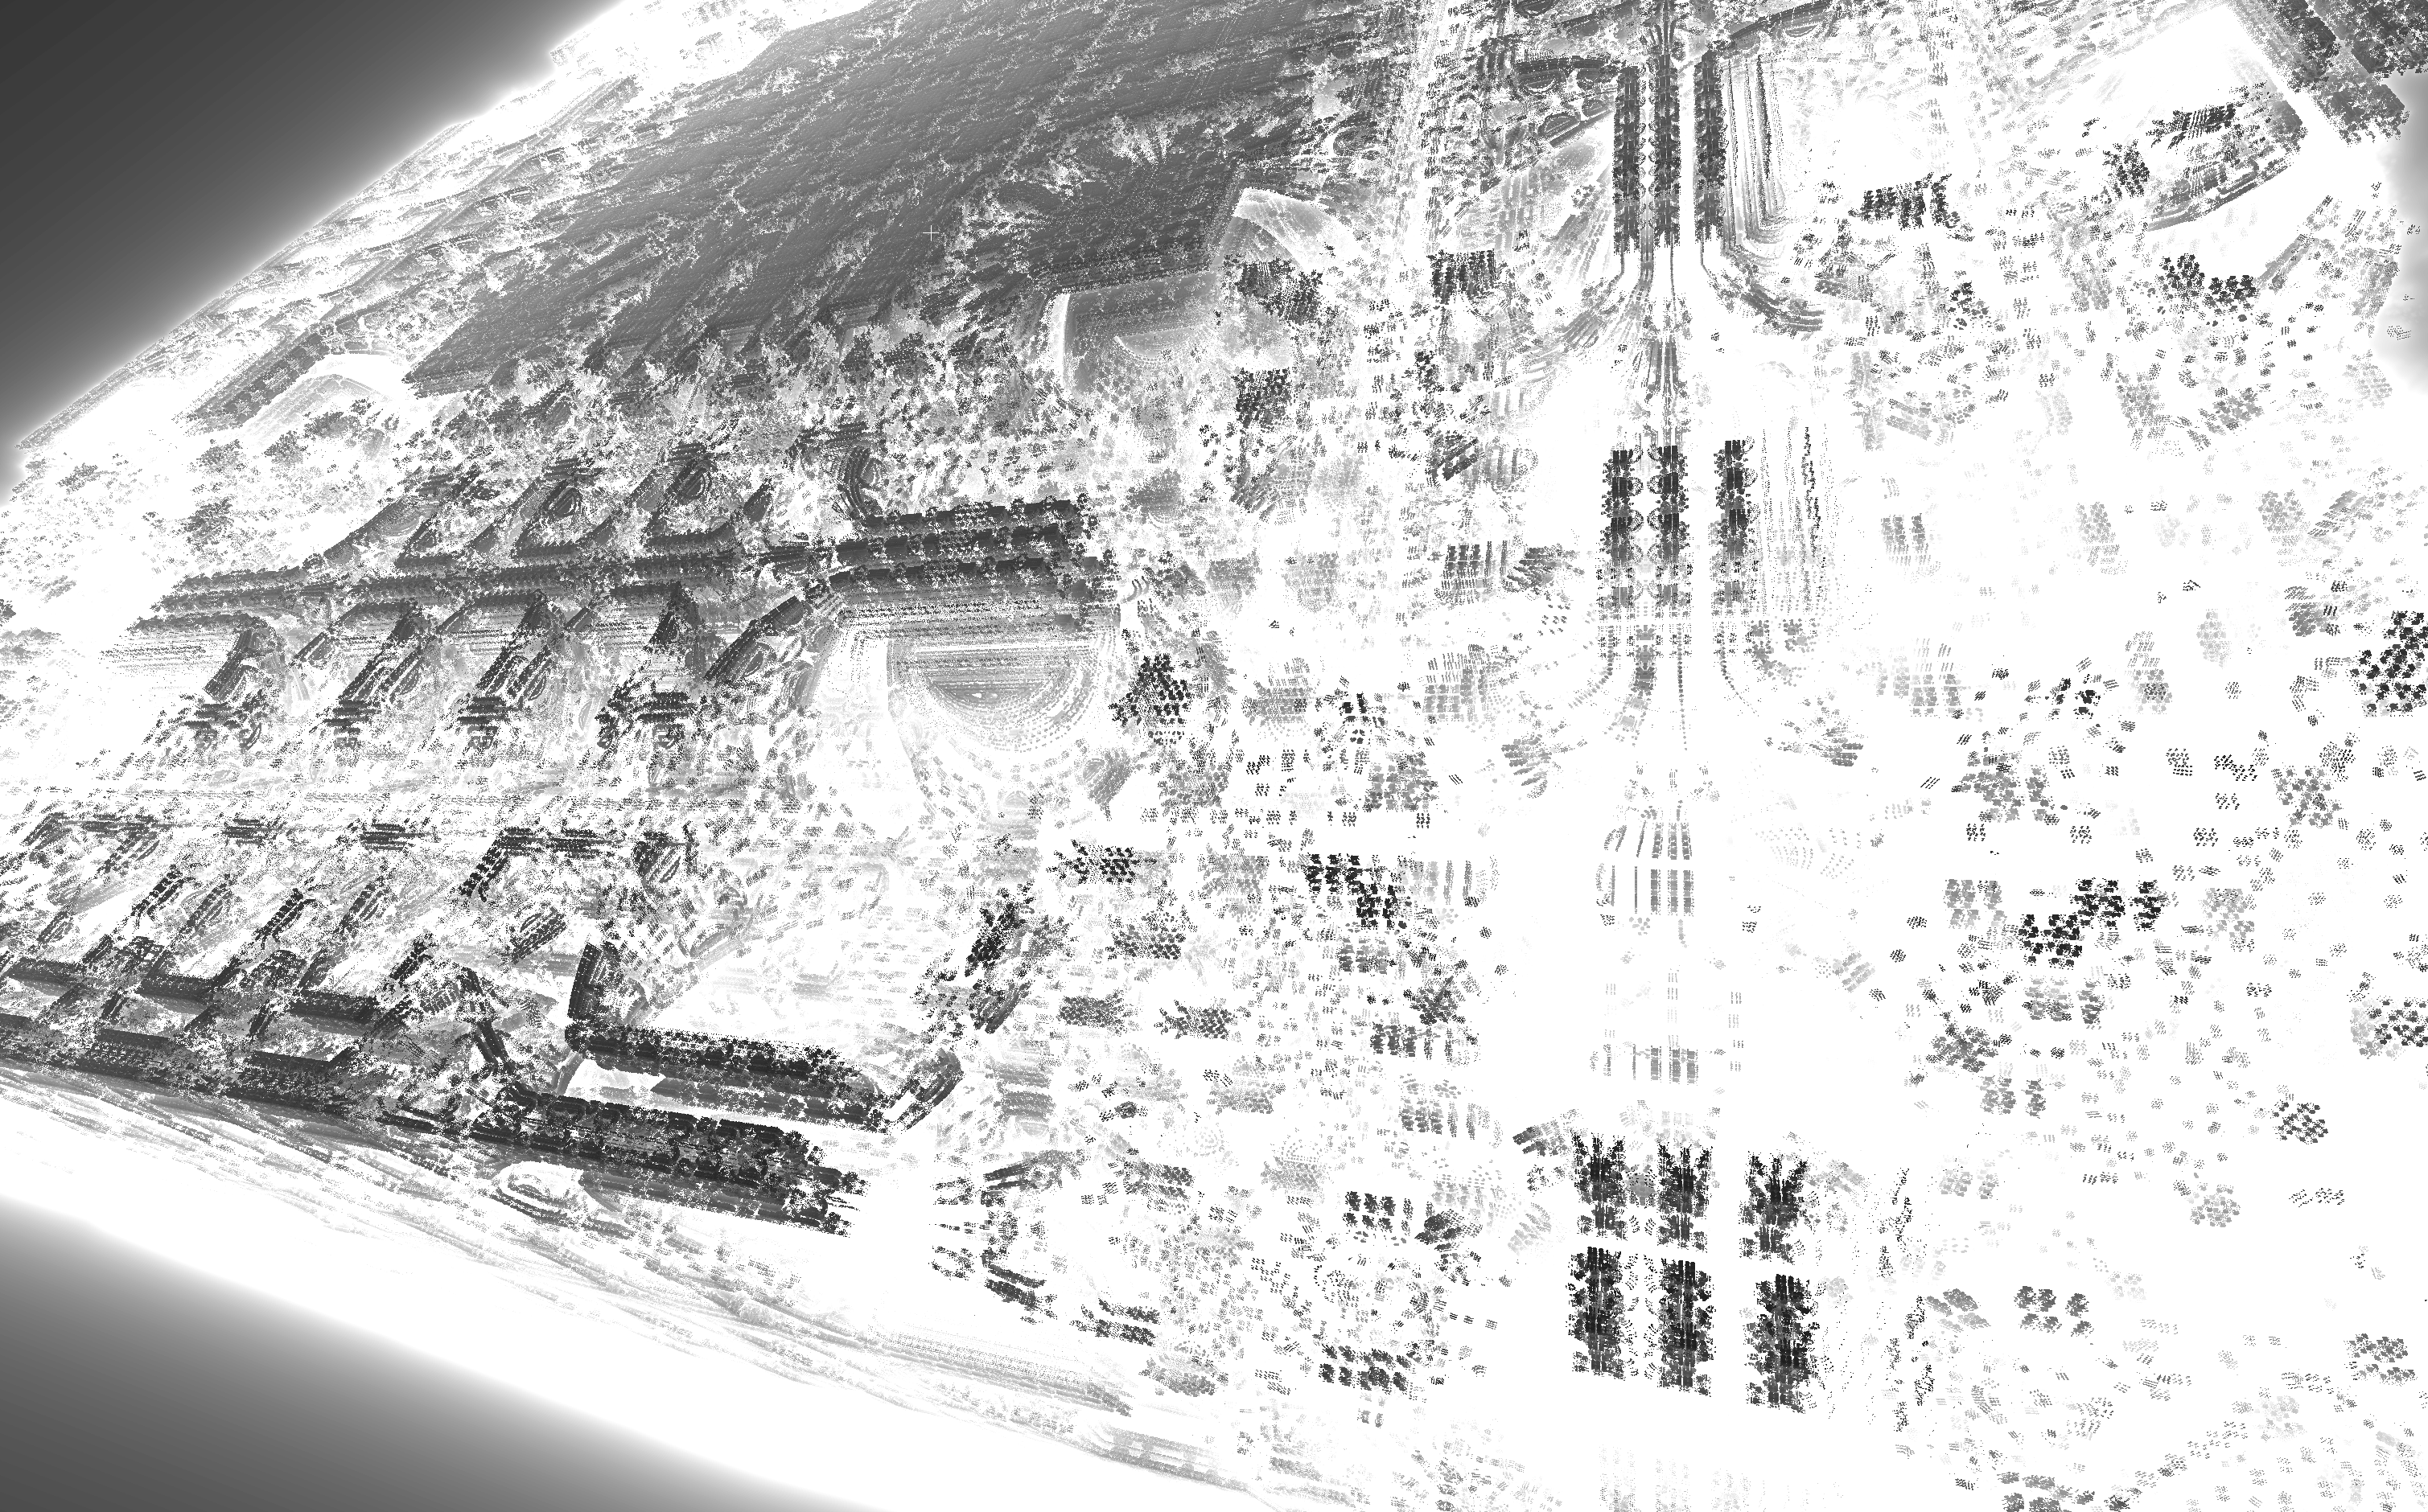
\includegraphics[width=\textwidth]{imgs/mandelbox_glsl_side.png}
        \label{fig:your_label}
    \end{minipage}
\end{center}

% ---------------------------------------------------------------
\subsection{Box Fold}
% ---------------------------------------------------------------

Each component of $\mathbf{v}$ is box-folded: if $|v_i| > 1$, it is reflected about
$\pm 1$:
%
\[
    \operatorname{BoxFold}(v_i) =
    \begin{cases}
        \phantom{-}2 - v_i  & \text{if } v_i > 1,  \\
        -2 - v_i             & \text{if } v_i < -1, \\
        \phantom{-}v_i       & \text{otherwise.}
    \end{cases}
\]

The fold limit acts as a container: reflections about $\pm1$ layer copies of space on top of each other, producing the self-similar nested structure characteristic of a fractal boundary.

% ---------------------------------------------------------------
\subsection{Sphere Fold}
% ---------------------------------------------------------------

The sphere fold prevents box-folded points near the origin from collapsing under scaling. Two concentric spheres ($m=0.5$, $f=1.0$) define three radial zones; points inside the inner sphere are repelled by inversion:
%
\[
    \mathbf{p}_{\text{out}} = \frac{f^{2}}{\|\mathbf{p}_{\text{in}}\|^{2}}\,\mathbf{p}_{\text{in}}.
\]
%
This smooths the sharp corners of the box fold into curved fractal boundaries.

\[
    \text{SphereFold}(\mathbf{v}) =
    \begin{cases}
        4\,\mathbf{v}                          & r^2 < m^2 \quad \text{(fixed scale; prevents underflow)} \\
        \mathbf{v}/r^2                         & m^2 \leq r^2 < f^2 \quad \text{(full inversion, } 1 < g < 4\text{)} \\
        \mathbf{v}                             & r^2 \geq f^2 \quad \text{(unchanged)}
    \end{cases}
\]

% ---------------------------------------------------------------
\subsection{Scaling, Translation and Derivatives}
% ---------------------------------------------------------------

Following the box and sphere folds, this step zooms towards the origin and shifts by
$\mathbf{c}$:
%
\[
    \mathbf{v}_{n+1} = s\,\mathbf{v}_{\text{folded}} + \mathbf{c},
\]
%
where $s$ is the scale factor and $\mathbf{c}$ is the original point. Zooming into folded
space over iterations produces finer scale and detail. A negative scale applies a uniform
scaling and reflection simultaneously. This alternating reflection, combined with the
subsequent box fold, creates the characteristic inside-out cubic symmetry of the Mandelbox.

To maintain the distance field estimate, the derivative magnitude $dr$ is updated in
parallel using the spherical scaling multiplier $g$:
%
\[
    dr_{n+1} = |s|\cdot g\cdot dr_{n} + 1.
\]

% ---------------------------------------------------------------



\subsection{Results}

\begin{table}[htbp]
\centering
\small
\caption{Timing results --- scaffold vs.\ Mandelbox}
\label{tab:timing}
{\renewcommand{\arraystretch}{1.3}
\begin{tabular}{lcc}
\toprule
\textbf{Metric} & \textbf{Scaffold} & \textbf{Mandelbox} \\
\midrule
\code{SDF\_LAT}   & 107 cycles & 230 cycles \\
Clock             & 125\,MHz   & 100\,MHz   \\
WNS               & $+3.170$\,ns & $+3.216$\,ns \\
Failing endpoints & 0 & 0 \\
\bottomrule
\end{tabular}}
\end{table}

\FloatBarrier

The Mandelbox required reducing the clock to 100\,MHz; the iterated fold logic
exceeds the 8\,ns timing budget at 125\,MHz due to the depth of the conditional
fold chain.

  % ---------------------------------------------------------------                                                         
  \subsection{SystemVerilog Implementation}                                                                                 
  % ---------------------------------------------------------------                                                         
                                                                                                                            
  The Mandelbox SDF is implemented as a fully pipelined \texttt{scene\_sdf}
  module in SystemVerilog. All arithmetic uses the project-wide FP27 custom
  float library (\texttt{fp\_add}, \texttt{fp\_mul}, \texttt{fp\_sub},
  \texttt{fp\_isqrt}). There are no loops or iterative feedback paths,
  each of the 4 Mandelbox iterations is unrolled as a distinct pipeline
  stage chained sequentially.

  \subsubsection*{Per-Iteration Pipeline (49 cycles)}

  Each iteration applies box fold $\to$ $r^2$ $\to$ sphere fold $\to$
  scale\,+\,offset in four stages:

  \begin{table}[h!]
  \centering
  \caption{Pipeline stages per Mandelbox iteration}
  \begin{tabular}{clr}
  \hline
  \textbf{Stage} & \textbf{Operation} & \textbf{Cycles} \\
  \hline
  A & Box fold: \texttt{fp\_clamp1} (comb.) $+$ \texttt{fp\_sub} $\times 3$ & 4 \\
  B & $r^2 = x^2+y^2+z^2$: \texttt{fp\_mul}$\times 3$ $+$ \texttt{fp\_add}$\times 2$ & 12 \\
  C & Sphere fold: \texttt{fp\_isqrt} $+$ \texttt{fp\_mul}$^2$ $+$ mux reg & 25 \\
  D & Scale $+$ offset: \texttt{fp\_mul}$\times 3$ $+$ \texttt{fp\_add}$\times 3$ & 8 \\
  \hline
  \textbf{Total} & & \textbf{49} \\
  \hline
  \end{tabular}
  \end{table}

  \noindent The box fold is combinatorial; \texttt{fp\_clamp1} examines
  bit\,[25:0] against the FP27 encoding of 1.0 and \texttt{fp\_times2}
  increments the exponent field by 1, both in zero cycles:

  \begin{verbatim}
  function automatic [26:0] fp_clamp1(input [26:0] a);
      fp_clamp1 = (a[25:0] > {8'h7F,18'h0}) ? {a[26],8'h7F,18'h0} : a;
  endfunction

  function automatic [26:0] fp_times2(input [26:0] a);
      fp_times2 = (a[25:18]==8'd0) ? 27'h0 : {a[26],a[25:18]+8'd1,a[17:0]};
  endfunction
  \end{verbatim}

  \noindent The sphere fold computes $1/r^2$ via \texttt{fp\_isqrt} followed
  by a squaring multiply, then selects between three zones at a registered mux:

  \begin{verbatim}
  //zone flags registered at cycle N+1 after r^2 arrives
  always @(posedge clk) begin
      inner_r <= (r2[25:0] < FP_0P25[25:0]); //r^2 < 0.25
      outer_r <= (r2[25:0] < FP_ONE[25:0]);  //r^2 < 1.0
  end

  //mux at cycle N+25
  always @(posedge clk) begin
      xs <= inner_r ? fp_times2(fp_times2(xf)) :  //x4
            outer_r ? x_outer                    :  //x/r^2
                      xf;                           //unchanged
  end
  \end{verbatim}

  \subsubsection*{Unrolled Iteration Timing}

  The four iterations are chained; companion signals use \texttt{state\_pipe}
  shift registers to maintain cycle-accurate alignment:

  \begin{table}[h!]
  \centering
  \caption{Cycle boundaries of each unrolled iteration}
  \begin{tabular}{lrr}
  \hline
  \textbf{Iteration} & \textbf{Input cycle} & \textbf{Output cycle} \\
  \hline
  Pre-register     & 0   & 1   \\
  Iteration 1      & 1   & 50  \\
  Iteration 2      & 50  & 99  \\
  Iteration 3      & 99  & 148 \\
  Iteration 4      & 148 & 197 \\
  \texttt{fp\_length} & 197 & 229 \\
  Scale $\times 0.2$  & 229 & 233 \\
  Output register     & 233 & 234 \\
  \hline
  \textbf{SDF\_LAT} & \multicolumn{2}{r}{\textbf{234 cycles}} \\
  \hline
  \end{tabular}
  \end{table}

  \noindent The distance estimate is $\|z_4\| \times 0.2$, a conservative
  lower bound on $\|z_4\|\,/\,|s|^4 = \|z_4\|\,/\,5.0625$. This prevents
  the ray marcher from overstepping near the fractal boundary. The constant
  0.2 is encoded exactly in FP27 as
  \texttt{\{1'b0,\,8'h7C,\,18'h26666\}}.

  The module uses 48 \texttt{fp\_mul} instances across 4 iterations (12 per
  iteration), consuming 48 DSP48E1 blocks on the Zynq-7020 which has 220
  available within budget.

% ===============================================================
\section{HDMI Output}
% ===============================================================

We implemented the initial HDMI output subsystem using an on-chip BRAM
framebuffer, establishing the display pipeline and providing the project's first
end-to-end proof that the PL could produce a visible image on the monitor.

\code{framebuffer\_bram.sv} implements a dual-port BRAM: one port accepts write
operations from the render pipeline; the second drives continuous scan-out for
\code{hdmi\_timing.sv}. \code{iter\_to\_rgb.sv} maps completed ray iteration
counts to 24-bit RGB using a pre-computed look-up table (\code{fog\_lut.mem}),
applying a fog gradient that serves as a perceptual depth cue. As discussed earlier, the BRAM framebuffer was replaced by AXI VDMA in the
final design, as the $1024 \times 600 \times 32$-bit frame (24.6\,Mbit) far
exceeds the available BRAM (4.9\,Mbit). The older colour mapping and timing
modules were retained.


% ===============================================================
\section{Audio FFT Pipeline}
% ===============================================================

\subsection{Design Evolution}
Initial design used Xilinx FFT IP with AXI-DMA to compute frequency
bands in hardware on the PL. As discussed in Section~1.4, this was replaced by
a software FFT on the host PC. The hardware FFT IP block design
(\code{audio\_fft.bd}) and \code{fft\_bridge.v} remain in the repository as
reference.

\subsection{Software FFT Pipeline}
A 1024-point FFT is computed per audio block at 44.1\,kHz using
\code{numpy.fft.rfft} on the host PC, with bin spacing
$\Delta f = 44100/1024 \approx 43.1$\,Hz.

\begin{table}[htbp]
\centering
\small
\caption{FFT frequency band definitions}
\label{tab:fft_bands}
{\renewcommand{\arraystretch}{1.3}
\begin{tabular}{lll}
\toprule
\textbf{Band} & \textbf{Frequency Range} & \textbf{FFT Bins} \\
\midrule
Bass   & ${\sim}43$--$215$\,Hz   & 1--5    \\
Mid    & ${\sim}215$--$2024$\,Hz & 5--47   \\
Treble & ${\sim}2024$--$8061$\,Hz & 47--187 \\
\bottomrule
\end{tabular}}
\end{table}

\FloatBarrier

Exponential smoothing/EMA lerp ($\alpha = 0.3$) is applied to each band. Overall RMS
amplitude, spectral centroid, zero-crossing rate, and a beat detection flag
(energy $> 1.5\times$ the 20-frame rolling mean) are also computed. All eleven
features are packed as IEEE\,754 floats and streamed to the PYNQ over TCP.

\subsection{Mapping to SDF Parameters}

\begin{table}[htbp]
\centering
\small
\caption{Audio feature to SDF parameter mapping}
\label{tab:audio_mapping}
{\renewcommand{\arraystretch}{1.3}
\begin{tabular}{lll}
\toprule
\textbf{Feature} & \textbf{SDF register} & \textbf{Hardware effect} \\
\midrule
Bass energy       & \code{sdf\_params[0]} (\code{cell\_sz}) & Space tiling period \\
Mid energy        & \code{sdf\_params[1]} (\code{b\_fp})    & Geometry arm half-length \\
Treble energy     & \code{sdf\_params[2]} (\code{e\_fp})    & Strut edge thickness \\
RMS               & Camera orbit radius                       & Camera pull-in/out \\
Spectral centroid & Camera $y$ offset                        & Camera height \\
\bottomrule
\end{tabular}}
\end{table}

\FloatBarrier

% =============================================================
  \section{IMU}
  % =============================================================                                                           
   
  The MPU-6050 IMU is polled at 100\,Hz via a custom MMIO driver accessing                                                  
  the AXI IIC core at \texttt{0x41600000}. Standard \texttt{smbus} tooling
  cannot be used as the I$^2$C bus is routed through the PL fabric rather
  than the PS I$^2$C controller.

  Orientation is tracked with a complementary filter:
  \[
    R \leftarrow \alpha\,(R + \omega\,\Delta t) + (1-\alpha)\,R_{\text{accel}},
    \qquad \alpha = 0.98
  \]
  The gyroscope term dominates (98\%), with 2\% accelerometer blending to
  correct long-term drift. Gram--Schmidt re-orthogonalisation is applied
  after every update to prevent floating-point rounding from skewing the
  lookat matrix over time:
  \[                                                                                                                        
    \hat{r}_0 = \frac{r_0}{\|r_0\|}, \qquad
    \hat{r}_1 = \frac{r_1 - (r_1 \cdot \hat{r}_0)\,\hat{r}_0}                                                               
                     {\|r_1 - (r_1 \cdot \hat{r}_0)\,\hat{r}_0\|}, \qquad
    \hat{r}_2 = \hat{r}_0 \times \hat{r}_1
  \]

  Movement impulses are projected onto the current rotation matrix columns
  rather than world axes:

  \begin{center}
  \begin{tabular}{ll}
  \hline
  \textbf{Key} & \textbf{Direction} \\
  \hline
  W / S        & $\pm R[:,2]$ (forward) \\
  A / D        & $\pm R[:,0]$ (right)   \\
  Space / C    & $\pm R[:,1]$ (up)      \\
  \hline
  \end{tabular}
  \end{center}

  This fixed a controls-inversion bug where translating in absolute world
  coordinates caused movement to reverse direction once the camera passed
  the scene origin.

% ===============================================================
\section{Neural SDF Training Pipeline}
% ===============================================================

\subsection{Motivation and Background}

An SDF returns the shortest distance from any 3D point to the nearest surface
boundary. Though closed-form analytic SDFs exist for simple shapes, no strict
formula is derivable for complex geometry such as fractals or organic meshes.
A Neural SDF approximates the SDF by training on sampled point-distance pairs;
the trained network can then be queried at any 3D coordinate.

\subsection{Network Architecture and Quantisation}

The chosen architecture is a $3\to32\to32\to32\to1$ MLP with ReLU activations.
ReLU reduces to an elementary comparator and multiplexer in hardware, eliminates
the vanishing gradient problem, and maintains unit gradient through all hidden
layers. No activation is applied to the output neuron, since signed distances
must be capable of representing negative values for interior points.

While 32 neurons per layer proved sufficient for simple geometry (sphere, torus),
complex fractal parameters required upgrading to 64 neurons. Weights are
quantised from \texttt{float32} to Q4.12 fixed-point: representable range
$\pm 8.0$, resolution $2^{-12} \approx 0.000244$.

\subsection{Training Pipeline}

Training data is generated by sampling 500,000 random points from $[-2, 2]^3$
and computing ground-truth SDF values analytically. The dataset is split 80/20
and trained with Adam optimiser and MSE loss in batches of 4096.

\subsection{Results}

\begin{table}[htbp]
\centering
\small
\caption{Neural SDF training results}
\label{tab:neural_results}
{\renewcommand{\arraystretch}{1.3}
\begin{tabular}{llc}
\toprule
\textbf{Shape} & \textbf{Architecture} & \textbf{Test Loss} \\
\midrule
Sphere    & $3\to32\to32\to32\to1$ & 0.000031 \\
Torus     & $3\to32\to32\to32\to1$ & 0.000053 \\
\bottomrule
\end{tabular}}
\end{table}

\FloatBarrier

\subsection{Weight Export}

Following training, weights are exported in Q4.12 hex format:
\begin{lstlisting}[language=Python]
format(int(round(w * 4096)) & 0xFFFF, '04x')
\end{lstlisting}
The 32-neuron network produces 260 files (\code{w\_\{layer\}\_\{neuron\}.hex},
\code{b\_\{layer\}\_\{neuron\}.hex}), directly parseable by Verilog
\code{\$readmemb}.


% ===============================================================
\section{Neural SDF Hardware Architecture}
\label{sec:neural_hw}
% ===============================================================

\subsection{Inference Engine Design}

Following the software training pipeline, it was proposed that the hardware inference
engine would consume the exported Q4.12 weights at synthesis time and
perform real-time MLP evaluation in the PL. The design comprises three modules:
\code{neuron\_layer.sv}, \code{sdf\_nn.sv}, and a trilinear interpolation cache
\code{trilinear\_interp.sv}.
Why Q4.12? 
Q4.12 was chosen as the weight format for three reasons.
First, each weight occupies a single 16-bit word, keeping BRAM usage half
that of \texttt{float32} weights.
Second, a 16-bit signed multiply fits natively into a single \texttt{DSP48E1}
18$\times$18 multiplier, the same primitive used throughout the FP27
library, whereas \texttt{float32} would require four DSP slices per weight
multiply.
Third, the four integer bits give a representable range of $[-8,\,8)$,
sufficient for the normalised weight magnitudes produced by the PyTorch
training pipeline, and the twelve fractional bits give a resolution of
$2^{-12}\approx2.4\times10^{-4}$, which was found adequate to keep inference
error below $0.5\%$ on the training geometry.

\code{neuron\_layer.sv} implements one fully connected layer. Weights for each
neuron are baked into BRAM at synthesis via \code{\$readmemb}, which reads the
hex files exported by the training script. The dot product is computed across
all input neurons in parallel using an array of Q4.12 fixed-point multipliers,
then accumulated with a final bias addition. A ReLU gate (implemented as a sign
bit comparator and output mux) is applied when the \code{USE\_RELU} parameter
is set; the output layer instantiates the module with \code{USE\_RELU = 0} to
allow signed distance outputs. For the 32-neuron hidden layers, 32 multipliers
run in parallel, accumulating into a 32-bit sum in $\log_2 32 = 5$ adder stages
(binary adder tree), plus one pipeline register per stage, giving a layer latency
of approximately 10 clock cycles.

\code{sdf\_nn.sv} chains three \code{neuron\_layer} instances (two hidden,
one output) and presents the same uniform interface as the analytic SDF modules
(inputs \code{px}, \code{py}, \code{pz}, output \code{sdf\_out}) allowing
it to be substituted into \code{march\_core} without any pipeline changes beyond
updating the \code{SDF\_LAT} parameter.

Crucially, the inference latency is fully deterministic. Every Q4.12
multiply-accumulate operation completes in a fixed number of clock cycles:
the parallel weight multiplications across all input neurons fire simultaneously,
their products are summed through a binary adder tree of fixed depth
$\lceil\log_2 N\rceil$ for $N$ inputs, a bias is added, and ReLU is applied
, all in a fixed pipeline with no data-dependent branching.
Chaining three such layers gives a total MLP latency that is a compile-time
constant, exactly as \code{SDF\_LAT} is for the analytic scenes.
The march pipeline makes no distinction between analytic and neural SDFs:
it simply waits \code{SDF\_LAT} cycles after presenting coordinates before
sampling the result, regardless of what is inside the SDF module.


\subsection{Trilinear Interpolation Cache}

The 3D coordinate space is partitioned into a coarse voxel grid (see as 32 x 32 x 32 cubes). At synthesis
the SDF is precomputed at each grid vertex and stored in BRAM (\code{trilinear\_interp.sv})- that's the baking approach.
At runtime, the eight vertices surrounding a query point are read from BRAM and
their SDF values are linearly interpolated along each axis in sequence, replacing
the full MLP forward pass with eight BRAM reads and 7 multiply-accumulate
operations. This is significantly cheaper than the full inference chain and was
intended as a performance/accuracy tradeoff for low-complexity scenes. Indeed, full SDF neural inference (initially opted for) would require a neural inference pass per march, which blows computational throughput.

\begin{figure}[h!]
\centering
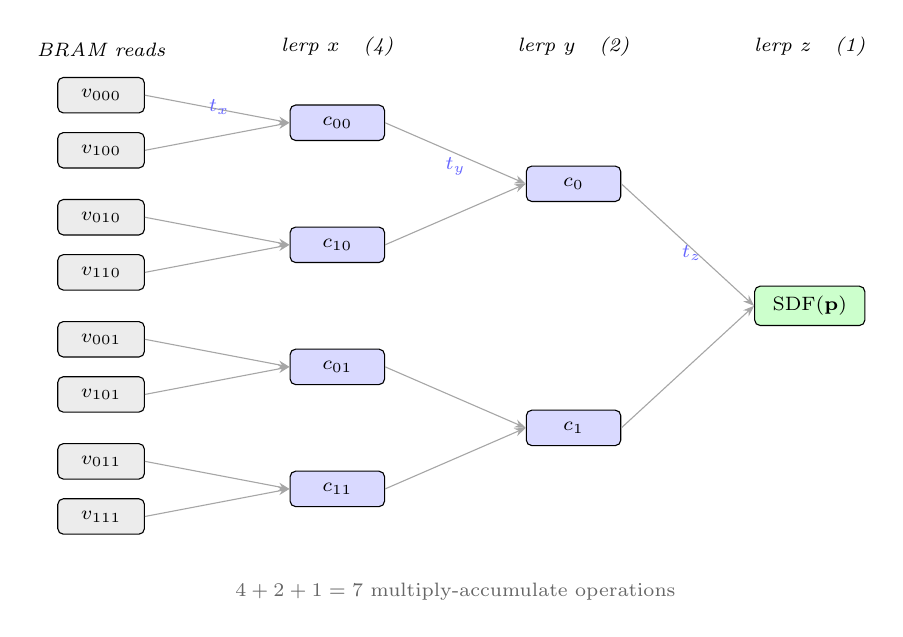
\begin{tikzpicture}[
  node distance=0.7cm,
  bram/.style={draw, fill=gray!15, rounded corners=2pt,
               minimum width=1.1cm, minimum height=0.45cm, font=\scriptsize},
  lerp/.style={draw, fill=blue!15, rounded corners=2pt,
               minimum width=1.2cm, minimum height=0.45cm, font=\scriptsize},
  res/.style={draw, fill=green!20, rounded corners=2pt,
              minimum width=1.4cm, minimum height=0.5cm, font=\scriptsize\bfseries},
  arr/.style={-{Stealth[length=4pt]}, gray!70},
  lbl/.style={font=\scriptsize\itshape},
]

%% ---- Column 0: BRAM reads (8 vertices) ----
\node[bram] (v000) at (0, 0.00) {$v_{000}$};
\node[bram] (v100) at (0,-0.70) {$v_{100}$};
\node[bram] (v010) at (0,-1.55) {$v_{010}$};
\node[bram] (v110) at (0,-2.25) {$v_{110}$};
\node[bram] (v001) at (0,-3.10) {$v_{001}$};
\node[bram] (v101) at (0,-3.80) {$v_{101}$};
\node[bram] (v011) at (0,-4.65) {$v_{011}$};
\node[bram] (v111) at (0,-5.35) {$v_{111}$};

\node[lbl, above=2pt] at (0, 0.3) {BRAM reads};

%% ---- Column 1: lerp along x (4 ops) ----
\node[lerp] (c00) at (3.0,-0.35) {$c_{00}$};
\node[lerp] (c10) at (3.0,-1.90) {$c_{10}$};
\node[lerp] (c01) at (3.0,-3.45) {$c_{01}$};
\node[lerp] (c11) at (3.0,-5.00) {$c_{11}$};

\node[lbl, above=2pt] at (3.0, 0.3) {lerp $x$\quad(4)};

\draw[arr] (v000.east) -- (c00.west);
\draw[arr] (v100.east) -- (c00.west);
\draw[arr] (v010.east) -- (c10.west);
\draw[arr] (v110.east) -- (c10.west);
\draw[arr] (v001.east) -- (c01.west);
\draw[arr] (v101.east) -- (c01.west);
\draw[arr] (v011.east) -- (c11.west);
\draw[arr] (v111.east) -- (c11.west);

%% ---- Column 2: lerp along y (2 ops) ----
\node[lerp] (cy0) at (6.0,-1.125) {$c_{0}$};
\node[lerp] (cy1) at (6.0,-4.225) {$c_{1}$};

\node[lbl, above=2pt] at (6.0, 0.3) {lerp $y$\quad(2)};

\draw[arr] (c00.east) -- (cy0.west);
\draw[arr] (c10.east) -- (cy0.west);
\draw[arr] (c01.east) -- (cy1.west);
\draw[arr] (c11.east) -- (cy1.west);

%% ---- Column 3: lerp along z (1 op) ----
\node[res] (result) at (9.0,-2.675) {$\mathrm{SDF}(\mathbf{p})$};

\node[lbl, above=2pt] at (9.0, 0.3) {lerp $z$\quad(1)};

\draw[arr] (cy0.east) -- (result.west);
\draw[arr] (cy1.east) -- (result.west);

%% ---- axis labels on edges ----
\node[lbl, color=blue!60] at (1.5,-0.15) {$t_x$};
\node[lbl, color=blue!60] at (4.5,-0.9) {$t_y$};
\node[lbl, color=blue!60] at (7.5,-2.0) {$t_z$};

%% ---- total op count ----
\node[font=\scriptsize, align=center, text=black!60]
  at (4.5,-6.3) {$4+2+1 = 7$ multiply-accumulate operations};

\end{tikzpicture}
\caption{Trilinear interpolation reduces eight BRAM-stored vertex SDF values
to a single query result in seven multiply-accumulate operations.
Interpolation weights $t_x,\,t_y,\,t_z \in [0,1]$ are the fractional
offsets of the query point within its voxel cell.}
\label{fig:trilinear}
\end{figure}

\begin{figure}[h!]
    \centering
    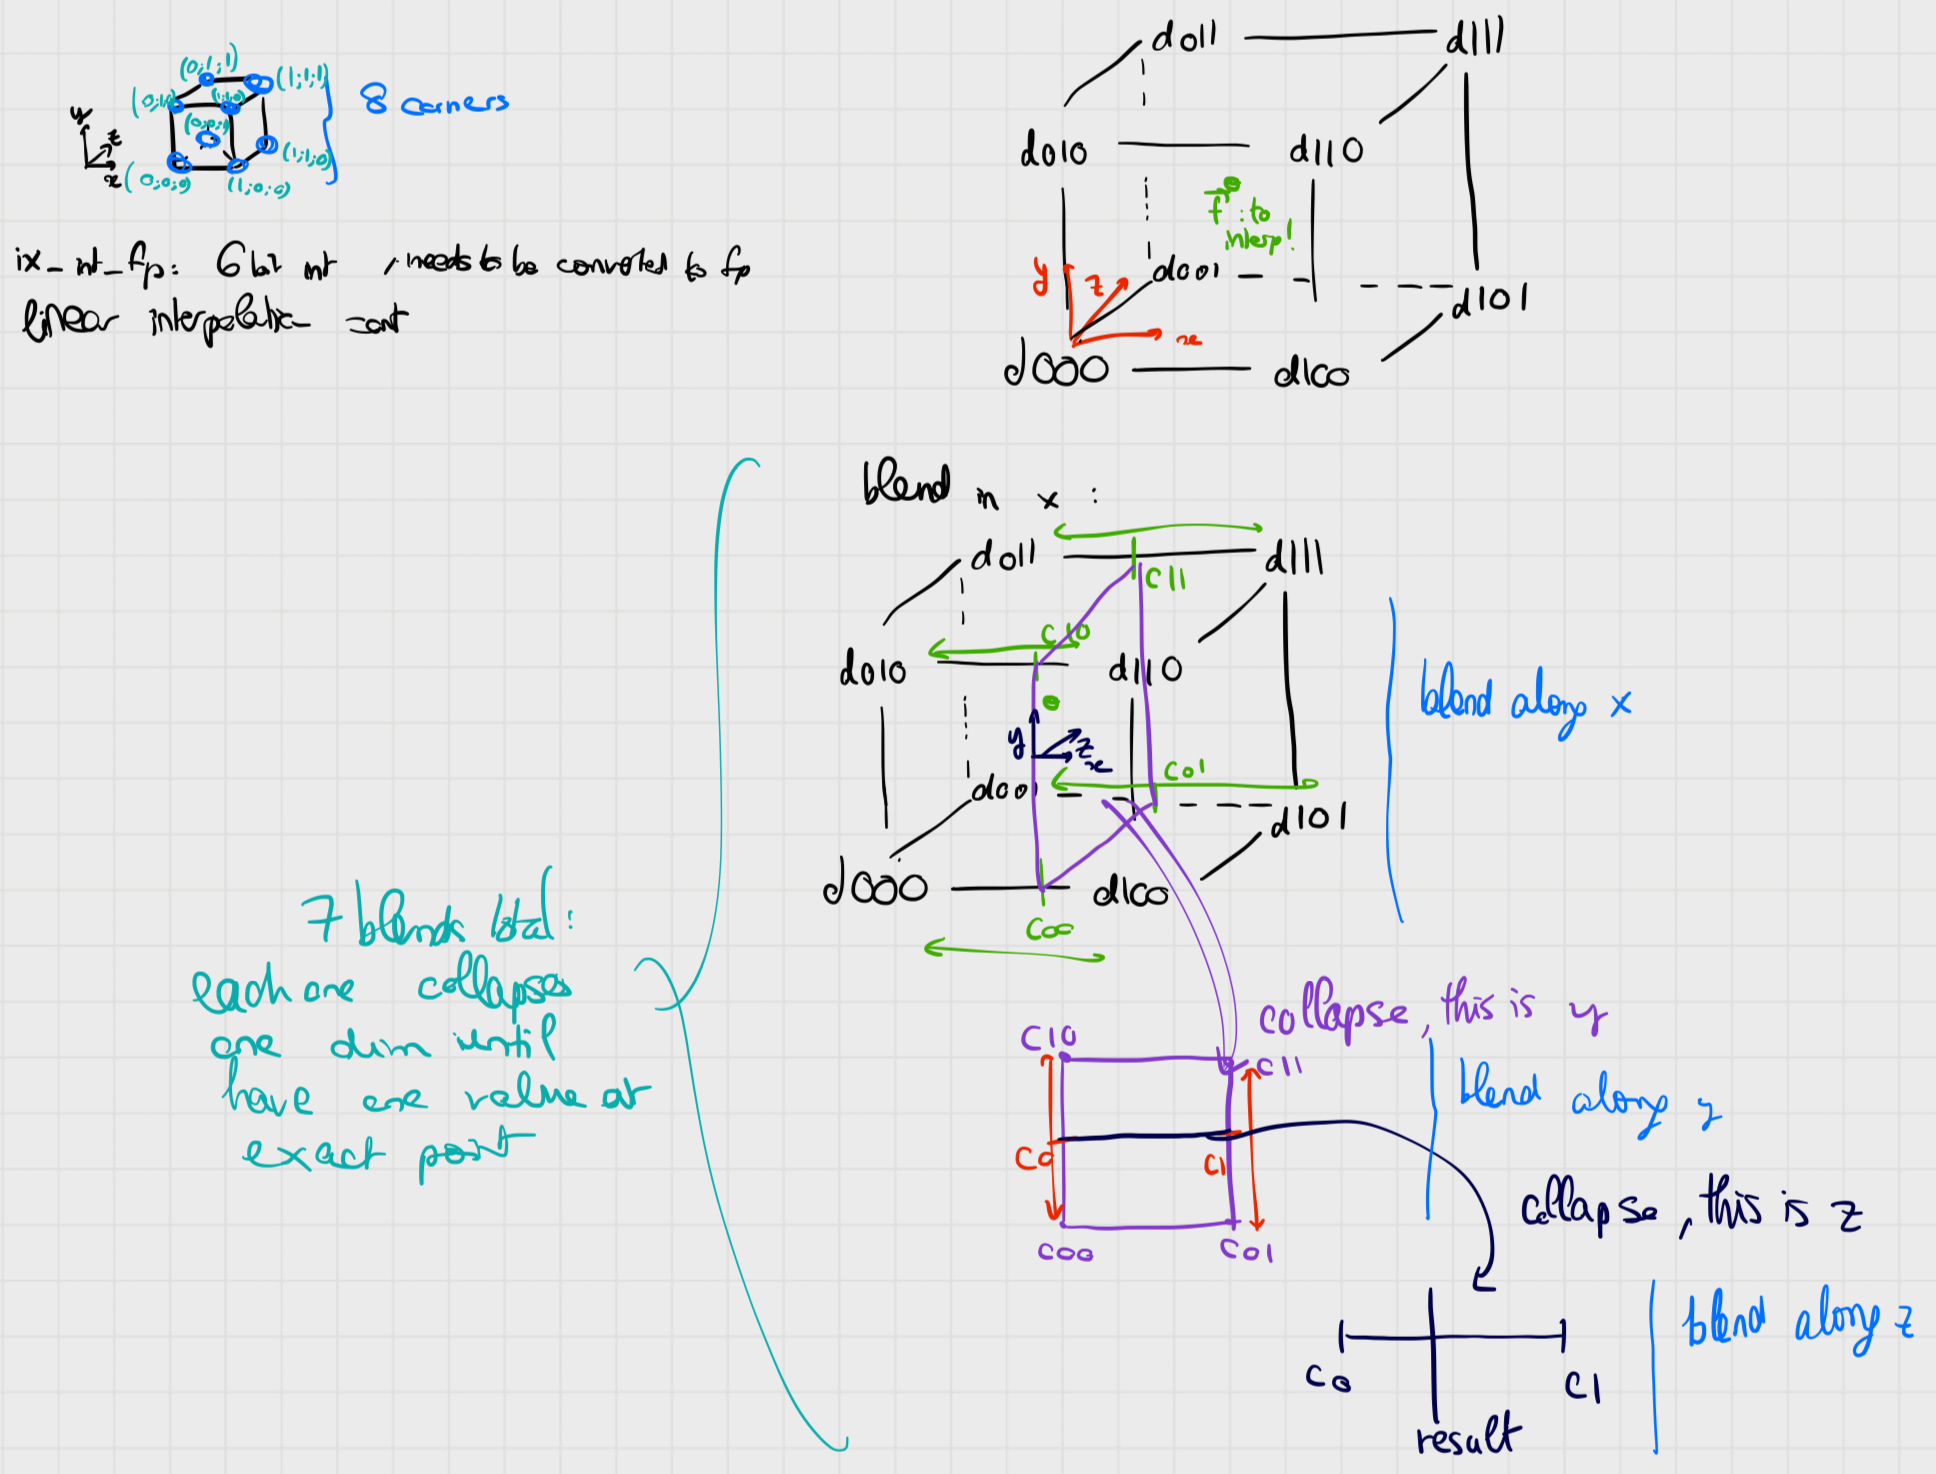
\includegraphics[width=0.8\textwidth]{imgs/lerp_visualized.png}
    \caption{A visual intuition as to how lerping is done in 3D}
    \label{fig:your_label}
\end{figure}

\subsection{Integration Status}

The training pipeline, weight export, and all hardware modules
(\code{neuron\_layer.sv}, \code{sdf\_nn.sv}, \code{trilinear\_interp.sv})
were implemented and synthesise without errors. The integration with
\code{march\_core} was not completed within the project timeline. The march
pipeline assumes a fixed-latency interface (one SDF result every clock cycle,
no backpressure). Since the MLP forward pass is fully pipelined with no
data-dependent branching, its latency is also a compile-time constant -
the fix is simply to count the pipeline stages across the three chained
\code{neuron\_layer} instances and set \code{SDF\_LAT} accordingly.
The integration was not completed within the project timeline and remains
as future work, but no architectural changes to \code{march\_core} are
required. Simply, it was feared that the DSP count on the PYNQ Z1 board could be easily exceeded when combining MLP + march core logic, as the single core version already consumed +30,000 LUTs and 140 DSPs. Pipelined use of DSPs would have to be considered, but we prefered to focus on the interactivity of our system through enhanced sound reactivity and smoother IMU control.



% ===============================================================
\section{Integrated Block Design and VDMA Pipeline}
\label{sec:vdma}
% ===============================================================

\subsection{Vivado Block Design}

The Vivado block design (\code{control\_bd.tcl}) connects all hardware subsystems.
The PS7 (ARM Cortex-A9) is the sole AXI-Lite master; it writes to the camera
register file and to the two AXI GPIO instances. On the high-performance path,
the AXI VDMA IP and the AXI framebuffer writer act as AXI4 masters, accessing
DDR3 through an AXI Interconnect that arbitrates between them and routes to the
PS7 HP slave port.

Key IP blocks:
\begin{itemize}
    \item \textbf{AXI VDMA}: reads completed frames from DDR3 and streams
    pixels to the RGB-to-DVI serialiser in park mode, looping on a fixed
    framebuffer.
    \item \textbf{rgb2dvi\_0}: converts 24-bit RGB pixel stream to TMDS
    differential pairs at 74.25\,MHz pixel clock.
    \item \textbf{clk\_wiz\_0}: generates 125\,MHz system clock and
    74.25\,MHz pixel clock from FCLK0 (50\,MHz from the PYNQ API).
    \item \textbf{AXI GPIO (0x41200000)}: two-channel GPIO for the
    frame-ready handshake: PL writes \code{frame\_ready\_valid} and
    \code{frame\_ready\_bank} on channel 1; PS writes \code{frame\_ack} on
    channel 2.
    \item \textbf{AXI GPIO (0x41210000)}: three push-button inputs read
    by the PS via MMIO for the scene selector UI.
\end{itemize}

\subsection{VDMA Double-Buffer Handshake}

The PL renders into one of two DDR3 framebuffers while the VDMA displays the
other. Frame synchronisation uses a two-signal AXI GPIO handshake implemented
in \code{ctrl.py}:

\begin{enumerate}
    \item PL finishes a complete frame, sets \code{frame\_ready\_valid = 1} and
    \code{frame\_ready\_bank = render\_bank}.
    \item PS polls the GPIO in \code{service\_frame\_ready()} and, on seeing
    \code{valid = 1}, calls \code{set\_display\_bank(vdma, ready\_bank)} to
    switch the VDMA park pointer to the completed buffer.
    \item PS pulses \code{frame\_ack = 1} for 1\,ms, then clears it.
    \item PL detects the ack, clears \code{frame\_ready\_valid}, and begins
    rendering the next frame into the other buffer.
\end{enumerate}

This handshake ensures no tearing: the VDMA pointer is updated only after a
complete frame is ready, and the PL does not overwrite a buffer while it is
being displayed.


\subsection{Integration Status}

The training pipeline, weight export, and all hardware modules
(\code{neuron\_layer.sv}, \code{sdf\_nn.sv}, \code{trilinear\_interp.sv})
were implemented and synthesise without errors. The integration with
\code{march\_core} was not completed within the project timeline. The march
pipeline assumes a fixed-latency interface (one SDF result every clock cycle,
no backpressure). Since the MLP forward pass is fully pipelined with no
data-dependent branching, its latency is also a compile-time constant -
the fix is simply to count the pipeline stages across the three chained
\code{neuron\_layer} instances and set \code{SDF\_LAT} accordingly.
The integration was not completed within the project timeline and remains
as future work, but no architectural changes to \code{march\_core} are
required. Simply, it was feared that the DSP count on the PYNQ Z1 board could be easily exceeded when combining MLP + march core logic, as the single core version already consumed +30,000 LUTs and 140 DSPs. Pipelined use of DSPs would have to be considered, but we prefered to focus on the interactivity of our system through enhanced sound reactivity and smoother IMU control.
